
% Default to the notebook output style

    


% Inherit from the specified cell style.




    
\documentclass[11pt]{article}

    
    
    \usepackage[T1]{fontenc}
    % Nicer default font (+ math font) than Computer Modern for most use cases
    \usepackage{mathpazo}

    % Basic figure setup, for now with no caption control since it's done
    % automatically by Pandoc (which extracts ![](path) syntax from Markdown).
    \usepackage{graphicx}
    % We will generate all images so they have a width \maxwidth. This means
    % that they will get their normal width if they fit onto the page, but
    % are scaled down if they would overflow the margins.
    \makeatletter
    \def\maxwidth{\ifdim\Gin@nat@width>\linewidth\linewidth
    \else\Gin@nat@width\fi}
    \makeatother
    \let\Oldincludegraphics\includegraphics
    % Set max figure width to be 80% of text width, for now hardcoded.
    \renewcommand{\includegraphics}[1]{\Oldincludegraphics[width=.8\maxwidth]{#1}}
    % Ensure that by default, figures have no caption (until we provide a
    % proper Figure object with a Caption API and a way to capture that
    % in the conversion process - todo).
    \usepackage{caption}
    \DeclareCaptionLabelFormat{nolabel}{}
    \captionsetup{labelformat=nolabel}

    \usepackage{adjustbox} % Used to constrain images to a maximum size 
    \usepackage{xcolor} % Allow colors to be defined
    \usepackage{enumerate} % Needed for markdown enumerations to work
    \usepackage{geometry} % Used to adjust the document margins
    \usepackage{amsmath} % Equations
    \usepackage{amssymb} % Equations
    \usepackage{textcomp} % defines textquotesingle
    % Hack from http://tex.stackexchange.com/a/47451/13684:
    \AtBeginDocument{%
        \def\PYZsq{\textquotesingle}% Upright quotes in Pygmentized code
    }
    \usepackage{upquote} % Upright quotes for verbatim code
    \usepackage{eurosym} % defines \euro
    \usepackage[mathletters]{ucs} % Extended unicode (utf-8) support
    \usepackage[utf8x]{inputenc} % Allow utf-8 characters in the tex document
    \usepackage{fancyvrb} % verbatim replacement that allows latex
    \usepackage{grffile} % extends the file name processing of package graphics 
                         % to support a larger range 
    % The hyperref package gives us a pdf with properly built
    % internal navigation ('pdf bookmarks' for the table of contents,
    % internal cross-reference links, web links for URLs, etc.)
    \usepackage{hyperref}
    \usepackage{longtable} % longtable support required by pandoc >1.10
    \usepackage{booktabs}  % table support for pandoc > 1.12.2
    \usepackage[inline]{enumitem} % IRkernel/repr support (it uses the enumerate* environment)
    \usepackage[normalem]{ulem} % ulem is needed to support strikethroughs (\sout)
                                % normalem makes italics be italics, not underlines
    

    
    
    % Colors for the hyperref package
    \definecolor{urlcolor}{rgb}{0,.145,.698}
    \definecolor{linkcolor}{rgb}{.71,0.21,0.01}
    \definecolor{citecolor}{rgb}{.12,.54,.11}

    % ANSI colors
    \definecolor{ansi-black}{HTML}{3E424D}
    \definecolor{ansi-black-intense}{HTML}{282C36}
    \definecolor{ansi-red}{HTML}{E75C58}
    \definecolor{ansi-red-intense}{HTML}{B22B31}
    \definecolor{ansi-green}{HTML}{00A250}
    \definecolor{ansi-green-intense}{HTML}{007427}
    \definecolor{ansi-yellow}{HTML}{DDB62B}
    \definecolor{ansi-yellow-intense}{HTML}{B27D12}
    \definecolor{ansi-blue}{HTML}{208FFB}
    \definecolor{ansi-blue-intense}{HTML}{0065CA}
    \definecolor{ansi-magenta}{HTML}{D160C4}
    \definecolor{ansi-magenta-intense}{HTML}{A03196}
    \definecolor{ansi-cyan}{HTML}{60C6C8}
    \definecolor{ansi-cyan-intense}{HTML}{258F8F}
    \definecolor{ansi-white}{HTML}{C5C1B4}
    \definecolor{ansi-white-intense}{HTML}{A1A6B2}

    % commands and environments needed by pandoc snippets
    % extracted from the output of `pandoc -s`
    \providecommand{\tightlist}{%
      \setlength{\itemsep}{0pt}\setlength{\parskip}{0pt}}
    \DefineVerbatimEnvironment{Highlighting}{Verbatim}{commandchars=\\\{\}}
    % Add ',fontsize=\small' for more characters per line
    \newenvironment{Shaded}{}{}
    \newcommand{\KeywordTok}[1]{\textcolor[rgb]{0.00,0.44,0.13}{\textbf{{#1}}}}
    \newcommand{\DataTypeTok}[1]{\textcolor[rgb]{0.56,0.13,0.00}{{#1}}}
    \newcommand{\DecValTok}[1]{\textcolor[rgb]{0.25,0.63,0.44}{{#1}}}
    \newcommand{\BaseNTok}[1]{\textcolor[rgb]{0.25,0.63,0.44}{{#1}}}
    \newcommand{\FloatTok}[1]{\textcolor[rgb]{0.25,0.63,0.44}{{#1}}}
    \newcommand{\CharTok}[1]{\textcolor[rgb]{0.25,0.44,0.63}{{#1}}}
    \newcommand{\StringTok}[1]{\textcolor[rgb]{0.25,0.44,0.63}{{#1}}}
    \newcommand{\CommentTok}[1]{\textcolor[rgb]{0.38,0.63,0.69}{\textit{{#1}}}}
    \newcommand{\OtherTok}[1]{\textcolor[rgb]{0.00,0.44,0.13}{{#1}}}
    \newcommand{\AlertTok}[1]{\textcolor[rgb]{1.00,0.00,0.00}{\textbf{{#1}}}}
    \newcommand{\FunctionTok}[1]{\textcolor[rgb]{0.02,0.16,0.49}{{#1}}}
    \newcommand{\RegionMarkerTok}[1]{{#1}}
    \newcommand{\ErrorTok}[1]{\textcolor[rgb]{1.00,0.00,0.00}{\textbf{{#1}}}}
    \newcommand{\NormalTok}[1]{{#1}}
    
    % Additional commands for more recent versions of Pandoc
    \newcommand{\ConstantTok}[1]{\textcolor[rgb]{0.53,0.00,0.00}{{#1}}}
    \newcommand{\SpecialCharTok}[1]{\textcolor[rgb]{0.25,0.44,0.63}{{#1}}}
    \newcommand{\VerbatimStringTok}[1]{\textcolor[rgb]{0.25,0.44,0.63}{{#1}}}
    \newcommand{\SpecialStringTok}[1]{\textcolor[rgb]{0.73,0.40,0.53}{{#1}}}
    \newcommand{\ImportTok}[1]{{#1}}
    \newcommand{\DocumentationTok}[1]{\textcolor[rgb]{0.73,0.13,0.13}{\textit{{#1}}}}
    \newcommand{\AnnotationTok}[1]{\textcolor[rgb]{0.38,0.63,0.69}{\textbf{\textit{{#1}}}}}
    \newcommand{\CommentVarTok}[1]{\textcolor[rgb]{0.38,0.63,0.69}{\textbf{\textit{{#1}}}}}
    \newcommand{\VariableTok}[1]{\textcolor[rgb]{0.10,0.09,0.49}{{#1}}}
    \newcommand{\ControlFlowTok}[1]{\textcolor[rgb]{0.00,0.44,0.13}{\textbf{{#1}}}}
    \newcommand{\OperatorTok}[1]{\textcolor[rgb]{0.40,0.40,0.40}{{#1}}}
    \newcommand{\BuiltInTok}[1]{{#1}}
    \newcommand{\ExtensionTok}[1]{{#1}}
    \newcommand{\PreprocessorTok}[1]{\textcolor[rgb]{0.74,0.48,0.00}{{#1}}}
    \newcommand{\AttributeTok}[1]{\textcolor[rgb]{0.49,0.56,0.16}{{#1}}}
    \newcommand{\InformationTok}[1]{\textcolor[rgb]{0.38,0.63,0.69}{\textbf{\textit{{#1}}}}}
    \newcommand{\WarningTok}[1]{\textcolor[rgb]{0.38,0.63,0.69}{\textbf{\textit{{#1}}}}}
    
    
    % Define a nice break command that doesn't care if a line doesn't already
    % exist.
    \def\br{\hspace*{\fill} \\* }
    % Math Jax compatability definitions
    \def\gt{>}
    \def\lt{<}
    % Document parameters
    \title{Python R training course - Session 2}
    
    
    

    % Pygments definitions
    
\makeatletter
\def\PY@reset{\let\PY@it=\relax \let\PY@bf=\relax%
    \let\PY@ul=\relax \let\PY@tc=\relax%
    \let\PY@bc=\relax \let\PY@ff=\relax}
\def\PY@tok#1{\csname PY@tok@#1\endcsname}
\def\PY@toks#1+{\ifx\relax#1\empty\else%
    \PY@tok{#1}\expandafter\PY@toks\fi}
\def\PY@do#1{\PY@bc{\PY@tc{\PY@ul{%
    \PY@it{\PY@bf{\PY@ff{#1}}}}}}}
\def\PY#1#2{\PY@reset\PY@toks#1+\relax+\PY@do{#2}}

\expandafter\def\csname PY@tok@cs\endcsname{\let\PY@it=\textit\def\PY@tc##1{\textcolor[rgb]{0.25,0.50,0.50}{##1}}}
\expandafter\def\csname PY@tok@sb\endcsname{\def\PY@tc##1{\textcolor[rgb]{0.73,0.13,0.13}{##1}}}
\expandafter\def\csname PY@tok@o\endcsname{\def\PY@tc##1{\textcolor[rgb]{0.40,0.40,0.40}{##1}}}
\expandafter\def\csname PY@tok@nv\endcsname{\def\PY@tc##1{\textcolor[rgb]{0.10,0.09,0.49}{##1}}}
\expandafter\def\csname PY@tok@dl\endcsname{\def\PY@tc##1{\textcolor[rgb]{0.73,0.13,0.13}{##1}}}
\expandafter\def\csname PY@tok@nb\endcsname{\def\PY@tc##1{\textcolor[rgb]{0.00,0.50,0.00}{##1}}}
\expandafter\def\csname PY@tok@gs\endcsname{\let\PY@bf=\textbf}
\expandafter\def\csname PY@tok@fm\endcsname{\def\PY@tc##1{\textcolor[rgb]{0.00,0.00,1.00}{##1}}}
\expandafter\def\csname PY@tok@sx\endcsname{\def\PY@tc##1{\textcolor[rgb]{0.00,0.50,0.00}{##1}}}
\expandafter\def\csname PY@tok@k\endcsname{\let\PY@bf=\textbf\def\PY@tc##1{\textcolor[rgb]{0.00,0.50,0.00}{##1}}}
\expandafter\def\csname PY@tok@gi\endcsname{\def\PY@tc##1{\textcolor[rgb]{0.00,0.63,0.00}{##1}}}
\expandafter\def\csname PY@tok@se\endcsname{\let\PY@bf=\textbf\def\PY@tc##1{\textcolor[rgb]{0.73,0.40,0.13}{##1}}}
\expandafter\def\csname PY@tok@kp\endcsname{\def\PY@tc##1{\textcolor[rgb]{0.00,0.50,0.00}{##1}}}
\expandafter\def\csname PY@tok@nd\endcsname{\def\PY@tc##1{\textcolor[rgb]{0.67,0.13,1.00}{##1}}}
\expandafter\def\csname PY@tok@vm\endcsname{\def\PY@tc##1{\textcolor[rgb]{0.10,0.09,0.49}{##1}}}
\expandafter\def\csname PY@tok@nf\endcsname{\def\PY@tc##1{\textcolor[rgb]{0.00,0.00,1.00}{##1}}}
\expandafter\def\csname PY@tok@go\endcsname{\def\PY@tc##1{\textcolor[rgb]{0.53,0.53,0.53}{##1}}}
\expandafter\def\csname PY@tok@mf\endcsname{\def\PY@tc##1{\textcolor[rgb]{0.40,0.40,0.40}{##1}}}
\expandafter\def\csname PY@tok@s\endcsname{\def\PY@tc##1{\textcolor[rgb]{0.73,0.13,0.13}{##1}}}
\expandafter\def\csname PY@tok@vi\endcsname{\def\PY@tc##1{\textcolor[rgb]{0.10,0.09,0.49}{##1}}}
\expandafter\def\csname PY@tok@vc\endcsname{\def\PY@tc##1{\textcolor[rgb]{0.10,0.09,0.49}{##1}}}
\expandafter\def\csname PY@tok@gp\endcsname{\let\PY@bf=\textbf\def\PY@tc##1{\textcolor[rgb]{0.00,0.00,0.50}{##1}}}
\expandafter\def\csname PY@tok@c\endcsname{\let\PY@it=\textit\def\PY@tc##1{\textcolor[rgb]{0.25,0.50,0.50}{##1}}}
\expandafter\def\csname PY@tok@si\endcsname{\let\PY@bf=\textbf\def\PY@tc##1{\textcolor[rgb]{0.73,0.40,0.53}{##1}}}
\expandafter\def\csname PY@tok@s2\endcsname{\def\PY@tc##1{\textcolor[rgb]{0.73,0.13,0.13}{##1}}}
\expandafter\def\csname PY@tok@ch\endcsname{\let\PY@it=\textit\def\PY@tc##1{\textcolor[rgb]{0.25,0.50,0.50}{##1}}}
\expandafter\def\csname PY@tok@kn\endcsname{\let\PY@bf=\textbf\def\PY@tc##1{\textcolor[rgb]{0.00,0.50,0.00}{##1}}}
\expandafter\def\csname PY@tok@w\endcsname{\def\PY@tc##1{\textcolor[rgb]{0.73,0.73,0.73}{##1}}}
\expandafter\def\csname PY@tok@cp\endcsname{\def\PY@tc##1{\textcolor[rgb]{0.74,0.48,0.00}{##1}}}
\expandafter\def\csname PY@tok@gt\endcsname{\def\PY@tc##1{\textcolor[rgb]{0.00,0.27,0.87}{##1}}}
\expandafter\def\csname PY@tok@na\endcsname{\def\PY@tc##1{\textcolor[rgb]{0.49,0.56,0.16}{##1}}}
\expandafter\def\csname PY@tok@cm\endcsname{\let\PY@it=\textit\def\PY@tc##1{\textcolor[rgb]{0.25,0.50,0.50}{##1}}}
\expandafter\def\csname PY@tok@mi\endcsname{\def\PY@tc##1{\textcolor[rgb]{0.40,0.40,0.40}{##1}}}
\expandafter\def\csname PY@tok@ni\endcsname{\let\PY@bf=\textbf\def\PY@tc##1{\textcolor[rgb]{0.60,0.60,0.60}{##1}}}
\expandafter\def\csname PY@tok@cpf\endcsname{\let\PY@it=\textit\def\PY@tc##1{\textcolor[rgb]{0.25,0.50,0.50}{##1}}}
\expandafter\def\csname PY@tok@gd\endcsname{\def\PY@tc##1{\textcolor[rgb]{0.63,0.00,0.00}{##1}}}
\expandafter\def\csname PY@tok@nc\endcsname{\let\PY@bf=\textbf\def\PY@tc##1{\textcolor[rgb]{0.00,0.00,1.00}{##1}}}
\expandafter\def\csname PY@tok@c1\endcsname{\let\PY@it=\textit\def\PY@tc##1{\textcolor[rgb]{0.25,0.50,0.50}{##1}}}
\expandafter\def\csname PY@tok@err\endcsname{\def\PY@bc##1{\setlength{\fboxsep}{0pt}\fcolorbox[rgb]{1.00,0.00,0.00}{1,1,1}{\strut ##1}}}
\expandafter\def\csname PY@tok@ow\endcsname{\let\PY@bf=\textbf\def\PY@tc##1{\textcolor[rgb]{0.67,0.13,1.00}{##1}}}
\expandafter\def\csname PY@tok@kr\endcsname{\let\PY@bf=\textbf\def\PY@tc##1{\textcolor[rgb]{0.00,0.50,0.00}{##1}}}
\expandafter\def\csname PY@tok@no\endcsname{\def\PY@tc##1{\textcolor[rgb]{0.53,0.00,0.00}{##1}}}
\expandafter\def\csname PY@tok@m\endcsname{\def\PY@tc##1{\textcolor[rgb]{0.40,0.40,0.40}{##1}}}
\expandafter\def\csname PY@tok@gu\endcsname{\let\PY@bf=\textbf\def\PY@tc##1{\textcolor[rgb]{0.50,0.00,0.50}{##1}}}
\expandafter\def\csname PY@tok@ge\endcsname{\let\PY@it=\textit}
\expandafter\def\csname PY@tok@s1\endcsname{\def\PY@tc##1{\textcolor[rgb]{0.73,0.13,0.13}{##1}}}
\expandafter\def\csname PY@tok@nn\endcsname{\let\PY@bf=\textbf\def\PY@tc##1{\textcolor[rgb]{0.00,0.00,1.00}{##1}}}
\expandafter\def\csname PY@tok@ss\endcsname{\def\PY@tc##1{\textcolor[rgb]{0.10,0.09,0.49}{##1}}}
\expandafter\def\csname PY@tok@nt\endcsname{\let\PY@bf=\textbf\def\PY@tc##1{\textcolor[rgb]{0.00,0.50,0.00}{##1}}}
\expandafter\def\csname PY@tok@sd\endcsname{\let\PY@it=\textit\def\PY@tc##1{\textcolor[rgb]{0.73,0.13,0.13}{##1}}}
\expandafter\def\csname PY@tok@mb\endcsname{\def\PY@tc##1{\textcolor[rgb]{0.40,0.40,0.40}{##1}}}
\expandafter\def\csname PY@tok@gh\endcsname{\let\PY@bf=\textbf\def\PY@tc##1{\textcolor[rgb]{0.00,0.00,0.50}{##1}}}
\expandafter\def\csname PY@tok@sr\endcsname{\def\PY@tc##1{\textcolor[rgb]{0.73,0.40,0.53}{##1}}}
\expandafter\def\csname PY@tok@gr\endcsname{\def\PY@tc##1{\textcolor[rgb]{1.00,0.00,0.00}{##1}}}
\expandafter\def\csname PY@tok@il\endcsname{\def\PY@tc##1{\textcolor[rgb]{0.40,0.40,0.40}{##1}}}
\expandafter\def\csname PY@tok@ne\endcsname{\let\PY@bf=\textbf\def\PY@tc##1{\textcolor[rgb]{0.82,0.25,0.23}{##1}}}
\expandafter\def\csname PY@tok@nl\endcsname{\def\PY@tc##1{\textcolor[rgb]{0.63,0.63,0.00}{##1}}}
\expandafter\def\csname PY@tok@kc\endcsname{\let\PY@bf=\textbf\def\PY@tc##1{\textcolor[rgb]{0.00,0.50,0.00}{##1}}}
\expandafter\def\csname PY@tok@bp\endcsname{\def\PY@tc##1{\textcolor[rgb]{0.00,0.50,0.00}{##1}}}
\expandafter\def\csname PY@tok@kd\endcsname{\let\PY@bf=\textbf\def\PY@tc##1{\textcolor[rgb]{0.00,0.50,0.00}{##1}}}
\expandafter\def\csname PY@tok@sc\endcsname{\def\PY@tc##1{\textcolor[rgb]{0.73,0.13,0.13}{##1}}}
\expandafter\def\csname PY@tok@sa\endcsname{\def\PY@tc##1{\textcolor[rgb]{0.73,0.13,0.13}{##1}}}
\expandafter\def\csname PY@tok@vg\endcsname{\def\PY@tc##1{\textcolor[rgb]{0.10,0.09,0.49}{##1}}}
\expandafter\def\csname PY@tok@kt\endcsname{\def\PY@tc##1{\textcolor[rgb]{0.69,0.00,0.25}{##1}}}
\expandafter\def\csname PY@tok@mo\endcsname{\def\PY@tc##1{\textcolor[rgb]{0.40,0.40,0.40}{##1}}}
\expandafter\def\csname PY@tok@sh\endcsname{\def\PY@tc##1{\textcolor[rgb]{0.73,0.13,0.13}{##1}}}
\expandafter\def\csname PY@tok@mh\endcsname{\def\PY@tc##1{\textcolor[rgb]{0.40,0.40,0.40}{##1}}}

\def\PYZbs{\char`\\}
\def\PYZus{\char`\_}
\def\PYZob{\char`\{}
\def\PYZcb{\char`\}}
\def\PYZca{\char`\^}
\def\PYZam{\char`\&}
\def\PYZlt{\char`\<}
\def\PYZgt{\char`\>}
\def\PYZsh{\char`\#}
\def\PYZpc{\char`\%}
\def\PYZdl{\char`\$}
\def\PYZhy{\char`\-}
\def\PYZsq{\char`\'}
\def\PYZdq{\char`\"}
\def\PYZti{\char`\~}
% for compatibility with earlier versions
\def\PYZat{@}
\def\PYZlb{[}
\def\PYZrb{]}
\makeatother


    % Exact colors from NB
    \definecolor{incolor}{rgb}{0.0, 0.0, 0.5}
    \definecolor{outcolor}{rgb}{0.545, 0.0, 0.0}



    
    % Prevent overflowing lines due to hard-to-break entities
    \sloppy 
    % Setup hyperref package
    \hypersetup{
      breaklinks=true,  % so long urls are correctly broken across lines
      colorlinks=true,
      urlcolor=urlcolor,
      linkcolor=linkcolor,
      citecolor=citecolor,
      }
    % Slightly bigger margins than the latex defaults
    
    \geometry{verbose,tmargin=1in,bmargin=1in,lmargin=1in,rmargin=1in}
    
    

    \begin{document}
    
    
    \maketitle
    
    

    
    \textbf{Lecture list}

\begin{enumerate}
\def\labelenumi{\arabic{enumi}.}
\item
  Introduction to Python
\item
  \textbf{The Python Standard Library, if/loops statements}

  \begin{itemize}
  \tightlist
  \item
    Some useful and basic built-in functions (abs, etc.)
  \item
    How to use import to import libraries (ex: math, random). We will
    introduce you several basic libraries that are often used in Python.
  \item
    Introduce Comparison and Boolean Operators (if/else/while/for)
  \item
    Students are also introduced the concept of object-orientation in
    Python.
  \end{itemize}
\item
  Vector/matrix structures, \texttt{numpy} library
\item
  Python data types, File Processing, \texttt{Pandas} library
\item
  Functions in Python, Debugging.
\item
  Introduction to R, R for Python programmers.
\item
  Import data, plot data.
\item
  Data Mining in Python/R.
\end{enumerate}

    \section{Some useful and basic built-in
functions}\label{some-useful-and-basic-built-in-functions}

List build-in functions:
\url{https://docs.python.org/2/library/functions.html}

\begin{figure}
\centering
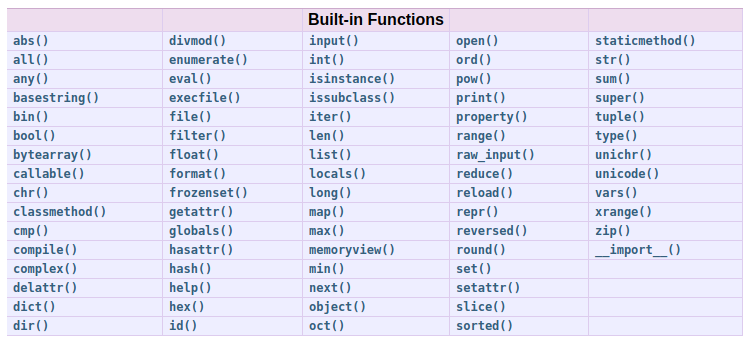
\includegraphics{figs/session_2/buildin-function.png}
\caption{}
\end{figure}

\begin{itemize}
\tightlist
\item
  \textbf{str()} is very common and useful for converting to strings,
  e.g. the number 1 to "1" -\/- similarily int() for converting other
  numbers (float or decimal), or strings, to integers.
\item
  \textbf{len()} is perhaps most common, we often need to know how many
  members there are e.g. in a list and len(mylist) is the Python way for
  that (not like mylist.length in Javascript)
\item
  \textbf{open()} is essential as that's what you use to open a file.
\item
  \textbf{min()} and \textbf{max()} are common. also \textbf{all()} and
  \textbf{any()} are handy to know for basic logic.
\item
  \textbf{set()} is useful because the set type doesn't have a literal
  like \textbf{{[}{]}} and \textbf{\{\}} for lists and dicts.
  \textbf{list()} is useful and quite common for converting e.g. a set
  to a list.
\item
  \textbf{range()} for iterating number of times:
  \texttt{for\ i\ in\ range(10)}
\item
  \textbf{sorted()} - creates sorted copy of list
\item
  \textbf{help({[}object{]})} - To invoke the built-in help.
\end{itemize}

    \subsection{Help}\label{help}

    \begin{Verbatim}[commandchars=\\\{\}]
{\color{incolor}In [{\color{incolor}1}]:} \PY{n}{help}\PY{p}{(}\PY{n+nb}{range}\PY{p}{)}
\end{Verbatim}


    \begin{Verbatim}[commandchars=\\\{\}]
Help on built-in function range in module \_\_builtin\_\_:

range({\ldots})
    range(stop) -> list of integers
    range(start, stop[, step]) -> list of integers
    
    Return a list containing an arithmetic progression of integers.
    range(i, j) returns [i, i+1, i+2, {\ldots}, j-1]; start (!) defaults to 0.
    When step is given, it specifies the increment (or decrement).
    For example, range(4) returns [0, 1, 2, 3].  The end point is omitted!
    These are exactly the valid indices for a list of 4 elements.


    \end{Verbatim}

    \subsection{Type conversion \& Type
coercion}\label{type-conversion-type-coercion}

Python provides a collection of built-in functions that convert values
from one type to another.

\begin{Shaded}
\begin{Highlighting}[]
\OperatorTok{>>>} \BuiltInTok{int}\NormalTok{(}\FloatTok{5.6}\NormalTok{)}
    \DecValTok{5}
    
\OperatorTok{>>>} \BuiltInTok{float}\NormalTok{(}\DecValTok{6}\NormalTok{)}
    \FloatTok{6.0}
    
\OperatorTok{>>>} \StringTok{'Two, '} \OperatorTok{+} \BuiltInTok{str}\NormalTok{(}\DecValTok{2}\NormalTok{)}
    \CommentTok{'Two, 2'}
    
\OperatorTok{>>>} \BuiltInTok{bool}\NormalTok{(}\DecValTok{6}\NormalTok{)}
    \VariableTok{True}
\NormalTok{    ...}
\end{Highlighting}
\end{Shaded}

    \subsection{Math}\label{math}

    \begin{Verbatim}[commandchars=\\\{\}]
{\color{incolor}In [{\color{incolor}2}]:} \PY{n+nb}{max}\PY{p}{(}\PY{l+m+mi}{91}\PY{p}{,} \PY{l+m+mi}{100}\PY{p}{)}
\end{Verbatim}


\begin{Verbatim}[commandchars=\\\{\}]
{\color{outcolor}Out[{\color{outcolor}2}]:} 100
\end{Verbatim}
            
    \begin{Verbatim}[commandchars=\\\{\}]
{\color{incolor}In [{\color{incolor}3}]:} \PY{n+nb}{min}\PY{p}{(}\PY{l+m+mi}{57}\PY{p}{,} \PY{n+nb}{min}\PY{p}{(}\PY{l+m+mi}{24}\PY{p}{,} \PY{l+m+mi}{44}\PY{p}{)}\PY{p}{)}
\end{Verbatim}


\begin{Verbatim}[commandchars=\\\{\}]
{\color{outcolor}Out[{\color{outcolor}3}]:} 24
\end{Verbatim}
            
    \begin{Verbatim}[commandchars=\\\{\}]
{\color{incolor}In [{\color{incolor}4}]:} \PY{k}{for} \PY{n}{i} \PY{o+ow}{in} \PY{n+nb}{range}\PY{p}{(}\PY{l+m+mi}{5}\PY{p}{,} \PY{l+m+mi}{10}\PY{p}{)}\PY{p}{:}
            \PY{k}{print} \PY{n}{i} \PY{o}{*}\PY{o}{*} \PY{l+m+mi}{2}
\end{Verbatim}


    \begin{Verbatim}[commandchars=\\\{\}]
25
36
49
64
81

    \end{Verbatim}

    \begin{Verbatim}[commandchars=\\\{\}]
{\color{incolor}In [{\color{incolor}5}]:} \PY{n+nb}{range}\PY{p}{(}\PY{l+m+mi}{5}\PY{p}{,}\PY{l+m+mi}{20}\PY{p}{,} \PY{l+m+mi}{2}\PY{p}{)}
\end{Verbatim}


\begin{Verbatim}[commandchars=\\\{\}]
{\color{outcolor}Out[{\color{outcolor}5}]:} [5, 7, 9, 11, 13, 15, 17, 19]
\end{Verbatim}
            
    \begin{Verbatim}[commandchars=\\\{\}]
{\color{incolor}In [{\color{incolor}6}]:} \PY{n}{x} \PY{o}{=} \PY{p}{[}\PY{l+m+mi}{1}\PY{p}{,} \PY{l+m+mi}{2}\PY{p}{,} \PY{l+m+mi}{3}\PY{p}{,} \PY{l+m+mi}{4}\PY{p}{]}
        \PY{n}{y} \PY{o}{=} \PY{p}{[}\PY{l+s+s1}{\PYZsq{}}\PY{l+s+s1}{a}\PY{l+s+s1}{\PYZsq{}}\PY{p}{,} \PY{l+s+s1}{\PYZsq{}}\PY{l+s+s1}{b}\PY{l+s+s1}{\PYZsq{}}\PY{p}{,} \PY{l+s+s1}{\PYZsq{}}\PY{l+s+s1}{c}\PY{l+s+s1}{\PYZsq{}}\PY{p}{]}
        
        \PY{n+nb}{zip}\PY{p}{(}\PY{n}{x}\PY{p}{,} \PY{n}{y}\PY{p}{)}
\end{Verbatim}


\begin{Verbatim}[commandchars=\\\{\}]
{\color{outcolor}Out[{\color{outcolor}6}]:} [(1, 'a'), (2, 'b'), (3, 'c')]
\end{Verbatim}
            
    \begin{Verbatim}[commandchars=\\\{\}]
{\color{incolor}In [{\color{incolor}6}]:} \PY{n+nb}{sorted}\PY{p}{(}\PY{p}{[}\PY{l+m+mi}{5}\PY{p}{,}\PY{l+m+mi}{3}\PY{p}{,}\PY{l+m+mi}{2}\PY{p}{,}\PY{l+m+mi}{5}\PY{p}{,}\PY{l+m+mi}{7}\PY{p}{,}\PY{l+m+mi}{8}\PY{p}{]}\PY{p}{)}
\end{Verbatim}


\begin{Verbatim}[commandchars=\\\{\}]
{\color{outcolor}Out[{\color{outcolor}6}]:} [2, 3, 5, 5, 7, 8]
\end{Verbatim}
            
    \subsection{Strings}\label{strings}

We have seen three types: \texttt{int}, \texttt{float}, and
\texttt{string}. \textbf{Strings} are qualitatively different from the
other two because they are made up of smaller pieces - characters.

The bracket operator selects a single character from a string.

    \begin{Verbatim}[commandchars=\\\{\}]
{\color{incolor}In [{\color{incolor}7}]:} \PY{n}{fruit} \PY{o}{=} \PY{l+s+s2}{\PYZdq{}}\PY{l+s+s2}{banana}\PY{l+s+s2}{\PYZdq{}}
        \PY{n}{letter} \PY{o}{=} \PY{n}{fruit}\PY{p}{[}\PY{l+m+mi}{1}\PY{p}{]} 
        \PY{k}{print} \PY{n}{letter}
\end{Verbatim}


    \begin{Verbatim}[commandchars=\\\{\}]
a

    \end{Verbatim}

    \begin{Verbatim}[commandchars=\\\{\}]
{\color{incolor}In [{\color{incolor}7}]:} \PY{n+nb}{len}\PY{p}{(}\PY{p}{[}\PY{l+m+mi}{1}\PY{p}{,}\PY{l+m+mi}{2}\PY{p}{]}\PY{p}{)}
\end{Verbatim}


\begin{Verbatim}[commandchars=\\\{\}]
{\color{outcolor}Out[{\color{outcolor}7}]:} 2
\end{Verbatim}
            
    \begin{Verbatim}[commandchars=\\\{\}]
{\color{incolor}In [{\color{incolor}9}]:} \PY{k}{for} \PY{n}{i} \PY{o+ow}{in} \PY{n+nb}{range}\PY{p}{(}\PY{n+nb}{len}\PY{p}{(}\PY{n}{fruit}\PY{p}{)}\PY{p}{)}\PY{p}{:}
            \PY{k}{print} \PY{l+s+s1}{\PYZsq{}}\PY{l+s+s1}{Char at}\PY{l+s+s1}{\PYZsq{}}\PY{p}{,} \PY{n}{i}\PY{p}{,} \PY{l+s+s1}{\PYZsq{}}\PY{l+s+s1}{is}\PY{l+s+s1}{\PYZsq{}}\PY{p}{,} \PY{n}{fruit}\PY{p}{[}\PY{n}{i}\PY{p}{]}
\end{Verbatim}


    \begin{Verbatim}[commandchars=\\\{\}]
Char at 0 is b
Char at 1 is a
Char at 2 is n
Char at 3 is a
Char at 4 is n
Char at 5 is a

    \end{Verbatim}

    \textbf{String slices}

The "slice" syntax is a handy way to refer to sub-parts of sequences
-\/- typically strings and lists. The slice s{[}start:end{]} is the
elements beginning at start and extending up to but not including end.
Suppose we have s = "Hello"

\begin{figure}
\centering
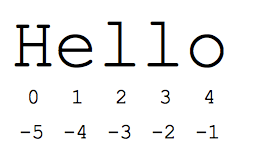
\includegraphics{figs/session_2/hello.png}
\caption{}
\end{figure}

    \begin{Verbatim}[commandchars=\\\{\}]
{\color{incolor}In [{\color{incolor}9}]:} \PY{n}{s} \PY{o}{=} \PY{l+s+s2}{\PYZdq{}}\PY{l+s+s2}{Hello}\PY{l+s+s2}{\PYZdq{}}
\end{Verbatim}


    \begin{Verbatim}[commandchars=\\\{\}]
{\color{incolor}In [{\color{incolor}18}]:} \PY{k}{print} \PY{n}{s}\PY{p}{[}\PY{o}{\PYZhy{}}\PY{l+m+mi}{1}\PY{p}{:}\PY{o}{\PYZhy{}}\PY{l+m+mi}{4}\PY{p}{]}
\end{Verbatim}


    \begin{Verbatim}[commandchars=\\\{\}]
oll

    \end{Verbatim}

    \begin{Verbatim}[commandchars=\\\{\}]
{\color{incolor}In [{\color{incolor}27}]:} \PY{n}{s}\PY{p}{[}\PY{l+m+mi}{4}\PY{p}{:}\PY{l+m+mi}{1}\PY{p}{:}\PY{o}{\PYZhy{}}\PY{l+m+mi}{1}\PY{p}{]}
\end{Verbatim}


\begin{Verbatim}[commandchars=\\\{\}]
{\color{outcolor}Out[{\color{outcolor}27}]:} 'oll'
\end{Verbatim}
            
    \begin{Verbatim}[commandchars=\\\{\}]
{\color{incolor}In [{\color{incolor}28}]:} \PY{n}{s}\PY{p}{[}\PY{o}{\PYZhy{}}\PY{l+m+mi}{4}\PY{p}{:}\PY{o}{\PYZhy{}}\PY{l+m+mi}{1}\PY{p}{]}
\end{Verbatim}


\begin{Verbatim}[commandchars=\\\{\}]
{\color{outcolor}Out[{\color{outcolor}28}]:} 'ell'
\end{Verbatim}
            
    \begin{Verbatim}[commandchars=\\\{\}]
{\color{incolor}In [{\color{incolor}25}]:} \PY{n}{s}\PY{p}{[}\PY{p}{:}\PY{p}{:}\PY{o}{\PYZhy{}}\PY{l+m+mi}{1}\PY{p}{]}
\end{Verbatim}


\begin{Verbatim}[commandchars=\\\{\}]
{\color{outcolor}Out[{\color{outcolor}25}]:} 'olle'
\end{Verbatim}
            
    \begin{Verbatim}[commandchars=\\\{\}]
{\color{incolor}In [{\color{incolor}29}]:} \PY{k}{print} \PY{n}{s}\PY{p}{[}\PY{o}{\PYZhy{}}\PY{l+m+mi}{1}\PY{p}{]}
\end{Verbatim}


    \begin{Verbatim}[commandchars=\\\{\}]
ll

    \end{Verbatim}

    \begin{Verbatim}[commandchars=\\\{\}]
{\color{incolor}In [{\color{incolor}5}]:} \PY{k}{print} \PY{n}{s}\PY{p}{[}\PY{o}{\PYZhy{}}\PY{l+m+mi}{4}\PY{p}{:}\PY{p}{]}
\end{Verbatim}


    \begin{Verbatim}[commandchars=\\\{\}]
ello

    \end{Verbatim}

    \begin{Verbatim}[commandchars=\\\{\}]
{\color{incolor}In [{\color{incolor}7}]:} \PY{n}{s}\PY{p}{[}\PY{p}{:}\PY{p}{:}\PY{o}{\PYZhy{}}\PY{l+m+mi}{1}\PY{p}{]}
\end{Verbatim}


\begin{Verbatim}[commandchars=\\\{\}]
{\color{outcolor}Out[{\color{outcolor}7}]:} 'olleH'
\end{Verbatim}
            
    \textbf{Exercise}

Ex1. Write a Python program to add 'ing' at the end of a given string
(length should be at least 3). If the given string already ends with
'ing' then add 'ly' instead. If the string length of the given string is
less than 3, leave it unchanged.

\begin{Shaded}
\begin{Highlighting}[]
\KeywordTok{def}\NormalTok{ add_string(s):}
    \CommentTok{# your code goes here}


\OperatorTok{>>>}\NormalTok{ add_string(}\StringTok{'abc'}\NormalTok{)}
    \CommentTok{'abcing'}
\OperatorTok{>>>}\NormalTok{ add_string(}\StringTok{'string'}\NormalTok{)}
    \CommentTok{'stringly'}
\end{Highlighting}
\end{Shaded}

    \begin{Verbatim}[commandchars=\\\{\}]
{\color{incolor}In [{\color{incolor}2}]:} \PY{c+c1}{\PYZsh{} Solution }
        \PY{k}{def} \PY{n+nf}{add\PYZus{}string}\PY{p}{(}\PY{n}{s}\PY{p}{)}\PY{p}{:}
            \PY{k}{if} \PY{n+nb}{len}\PY{p}{(}\PY{n}{s}\PY{p}{)} \PY{o}{\PYZlt{}} \PY{l+m+mi}{3}\PY{p}{:} \PY{k}{return} \PY{n}{s}
            \PY{k}{if} \PY{n}{s}\PY{p}{[}\PY{o}{\PYZhy{}}\PY{l+m+mi}{3}\PY{p}{:}\PY{p}{]} \PY{o}{==} \PY{l+s+s1}{\PYZsq{}}\PY{l+s+s1}{ing}\PY{l+s+s1}{\PYZsq{}}\PY{p}{:} \PY{k}{return} \PY{n}{s} \PY{o}{+} \PY{l+s+s1}{\PYZsq{}}\PY{l+s+s1}{ly}\PY{l+s+s1}{\PYZsq{}}
            \PY{k}{return} \PY{n}{s} \PY{o}{+} \PY{l+s+s1}{\PYZsq{}}\PY{l+s+s1}{ing}\PY{l+s+s1}{\PYZsq{}}
        
        \PY{k}{print} \PY{n}{add\PYZus{}string}\PY{p}{(}\PY{l+s+s1}{\PYZsq{}}\PY{l+s+s1}{string}\PY{l+s+s1}{\PYZsq{}}\PY{p}{)}
        \PY{k}{print} \PY{n}{add\PYZus{}string}\PY{p}{(}\PY{l+s+s1}{\PYZsq{}}\PY{l+s+s1}{abc}\PY{l+s+s1}{\PYZsq{}}\PY{p}{)}
\end{Verbatim}


    \begin{Verbatim}[commandchars=\\\{\}]
stringly
abcing

    \end{Verbatim}

    Ex2. Write a Python program to remove the nth index character from a
nonempty string.

Expect result

\begin{Shaded}
\begin{Highlighting}[]
\OperatorTok{>>>}\NormalTok{ remove_char(}\StringTok{'Python'}\NormalTok{, }\DecValTok{0}\NormalTok{)}
    \CommentTok{'ython'}
\OperatorTok{>>>}\NormalTok{ remove_char(}\StringTok{'Python'}\NormalTok{, }\DecValTok{3}\NormalTok{)}
    \CommentTok{'Pyton'}
\OperatorTok{>>>}\NormalTok{ remove_char(}\StringTok{'Python'}\NormalTok{, }\DecValTok{5}\NormalTok{)}
    \CommentTok{'Pytho'}
\end{Highlighting}
\end{Shaded}

    \begin{Verbatim}[commandchars=\\\{\}]
{\color{incolor}In [{\color{incolor}3}]:} \PY{c+c1}{\PYZsh{} Solution}
        \PY{k}{def} \PY{n+nf}{remove\PYZus{}char}\PY{p}{(}\PY{n}{s}\PY{p}{,} \PY{n}{index}\PY{p}{)}\PY{p}{:}
            \PY{k}{return} \PY{n}{s}\PY{p}{[}\PY{p}{:}\PY{n}{index}\PY{p}{]} \PY{o}{+} \PY{n}{s}\PY{p}{[}\PY{n}{index}\PY{o}{+}\PY{l+m+mi}{1}\PY{p}{:}\PY{p}{]}
        
        \PY{n}{remove\PYZus{}char}\PY{p}{(}\PY{l+s+s1}{\PYZsq{}}\PY{l+s+s1}{Python}\PY{l+s+s1}{\PYZsq{}}\PY{p}{,} \PY{l+m+mi}{0}\PY{p}{)}
\end{Verbatim}


\begin{Verbatim}[commandchars=\\\{\}]
{\color{outcolor}Out[{\color{outcolor}3}]:} 'ython'
\end{Verbatim}
            
    Ex3. Write a Python function to insert a string in the middle of a
string. Using \textbf{remove\_char()} function in Ex2 to remove the
middle char.

\begin{Shaded}
\begin{Highlighting}[]
\OperatorTok{>>>}\NormalTok{ insert_middle(}\StringTok{'}\SpecialCharTok{\{\{\}\}}\StringTok{'}\NormalTok{, }\StringTok{'JVN'}\NormalTok{)}
    \CommentTok{"\{\{JVN\}\}"}
    
\OperatorTok{>>>}\NormalTok{ insert_middle(}\StringTok{'[[x]]'}\NormalTok{, }\StringTok{'JVN'}\NormalTok{)}
    \CommentTok{"[[JVN]]}
\end{Highlighting}
\end{Shaded}

    \begin{Verbatim}[commandchars=\\\{\}]
{\color{incolor}In [{\color{incolor}7}]:} \PY{c+c1}{\PYZsh{} Solution}
        \PY{k}{def} \PY{n+nf}{insert\PYZus{}middle}\PY{p}{(}\PY{n}{s}\PY{p}{,} \PY{n}{sub\PYZus{}s}\PY{p}{)}\PY{p}{:}
            \PY{k}{if} \PY{n+nb}{len}\PY{p}{(}\PY{n}{s}\PY{p}{)} \PY{o}{\PYZpc{}} \PY{l+m+mi}{2} \PY{o}{==} \PY{l+m+mi}{1}\PY{p}{:}
                \PY{n}{s} \PY{o}{=} \PY{n}{remove\PYZus{}char}\PY{p}{(}\PY{n}{s}\PY{p}{,} \PY{n+nb}{len}\PY{p}{(}\PY{n}{s}\PY{p}{)}\PY{o}{/}\PY{l+m+mi}{2}\PY{p}{)}
            
            \PY{n}{middle\PYZus{}index} \PY{o}{=} \PY{n+nb}{len}\PY{p}{(}\PY{n}{s}\PY{p}{)} \PY{o}{/} \PY{l+m+mi}{2}
            \PY{k}{return} \PY{n}{s}\PY{p}{[}\PY{p}{:}\PY{n}{middle\PYZus{}index}\PY{p}{]} \PY{o}{+} \PY{n}{sub\PYZus{}s} \PY{o}{+} \PY{n}{s}\PY{p}{[}\PY{n}{middle\PYZus{}index}\PY{p}{:}\PY{p}{]}
        
        \PY{n}{insert\PYZus{}middle}\PY{p}{(}\PY{l+s+s1}{\PYZsq{}}\PY{l+s+s1}{[[x]]}\PY{l+s+s1}{\PYZsq{}}\PY{p}{,} \PY{l+s+s1}{\PYZsq{}}\PY{l+s+s1}{JVN}\PY{l+s+s1}{\PYZsq{}}\PY{p}{)}
\end{Verbatim}


\begin{Verbatim}[commandchars=\\\{\}]
{\color{outcolor}Out[{\color{outcolor}7}]:} '[[JVN]]'
\end{Verbatim}
            
    Ex4. Write a Python program to count the occurrences of each word in a
given sentence

\begin{Shaded}
\begin{Highlighting}[]
\OperatorTok{>>>}\NormalTok{ word_count(}\StringTok{'the quick brown fox jumps over the lazy dog'}\NormalTok{)}
\NormalTok{    \{}\StringTok{'the'}\NormalTok{: }\DecValTok{2}\NormalTok{, }\StringTok{'jumps'}\NormalTok{: }\DecValTok{1}\NormalTok{, }\StringTok{'brown'}\NormalTok{: }\DecValTok{1}\NormalTok{, }\StringTok{'lazy'}\NormalTok{: }\DecValTok{1}\NormalTok{, }\StringTok{'fox'}\NormalTok{: }\DecValTok{1}\NormalTok{, }\StringTok{'over'}\NormalTok{: }\DecValTok{1}\NormalTok{, }\StringTok{'quick'}\NormalTok{: }\DecValTok{1}\NormalTok{, }\StringTok{'dog'}\NormalTok{: }\DecValTok{1}\NormalTok{\} }
\end{Highlighting}
\end{Shaded}

    \begin{Verbatim}[commandchars=\\\{\}]
{\color{incolor}In [{\color{incolor}8}]:} \PY{k}{def} \PY{n+nf}{word\PYZus{}count}\PY{p}{(}\PY{n}{s}\PY{p}{)}\PY{p}{:}
            \PY{n}{s} \PY{o}{=} \PY{n}{s}\PY{o}{.}\PY{n}{split}\PY{p}{(}\PY{p}{)}
            \PY{n}{wc} \PY{o}{=} \PY{p}{\PYZob{}}\PY{p}{\PYZcb{}}
            \PY{k}{for} \PY{n}{word} \PY{o+ow}{in} \PY{n}{s}\PY{p}{:}
                \PY{n}{wc}\PY{p}{[}\PY{n}{word}\PY{p}{]} \PY{o}{=} \PY{n}{wc}\PY{o}{.}\PY{n}{get}\PY{p}{(}\PY{n}{word}\PY{p}{,} \PY{l+m+mi}{0}\PY{p}{)} \PY{o}{+} \PY{l+m+mi}{1}
            
            \PY{k}{return} \PY{n}{wc}
        
        \PY{n}{word\PYZus{}count}\PY{p}{(}\PY{l+s+s1}{\PYZsq{}}\PY{l+s+s1}{the quick brown fox jumps over the lazy dog}\PY{l+s+s1}{\PYZsq{}}\PY{p}{)}
\end{Verbatim}


\begin{Verbatim}[commandchars=\\\{\}]
{\color{outcolor}Out[{\color{outcolor}8}]:} \{'brown': 1,
         'dog': 1,
         'fox': 1,
         'jumps': 1,
         'lazy': 1,
         'over': 1,
         'quick': 1,
         'the': 2\}
\end{Verbatim}
            
    Ex5. Write a Python program to get the domain of URL

\begin{Shaded}
\begin{Highlighting}[]
\OperatorTok{>>>}\NormalTok{ get_domain(}\StringTok{"https://www.kaggle.com/wiki/Tutorials"}\NormalTok{)}
    \CommentTok{"www.kaggle.com"}
    
\OperatorTok{>>>}\NormalTok{ get_domain(}\StringTok{"http://www.kaggle.com/wiki/Tutorials"}\NormalTok{)}
    \CommentTok{"www.kaggle.com"}
    
\OperatorTok{>>>}\NormalTok{ get_domain(}\StringTok{"jvn.edu.vn/xyz"}\NormalTok{)}
    \CommentTok{"jvn.edu.vn"}
\end{Highlighting}
\end{Shaded}

Extras: * Using another library * Using regex to detect domain. Library
\texttt{re}

    \begin{Verbatim}[commandchars=\\\{\}]
{\color{incolor}In [{\color{incolor}10}]:} \PY{c+c1}{\PYZsh{} Solution 1}
         \PY{k}{def} \PY{n+nf}{get\PYZus{}domain}\PY{p}{(}\PY{n}{url} \PY{o}{=} \PY{l+s+s1}{\PYZsq{}}\PY{l+s+s1}{\PYZsq{}}\PY{p}{)}\PY{p}{:}
             \PY{n}{url} \PY{o}{=} \PY{n}{url}\PY{o}{.}\PY{n}{replace}\PY{p}{(}\PY{l+s+s1}{\PYZsq{}}\PY{l+s+s1}{http://}\PY{l+s+s1}{\PYZsq{}}\PY{p}{,} \PY{l+s+s1}{\PYZsq{}}\PY{l+s+s1}{\PYZsq{}}\PY{p}{)}\PY{o}{.}\PY{n}{replace}\PY{p}{(}\PY{l+s+s1}{\PYZsq{}}\PY{l+s+s1}{https://}\PY{l+s+s1}{\PYZsq{}}\PY{p}{,} \PY{l+s+s1}{\PYZsq{}}\PY{l+s+s1}{\PYZsq{}}\PY{p}{)}
             \PY{k}{return} \PY{n}{url}\PY{o}{.}\PY{n}{split}\PY{p}{(}\PY{l+s+s1}{\PYZsq{}}\PY{l+s+s1}{/}\PY{l+s+s1}{\PYZsq{}}\PY{p}{)}\PY{p}{[}\PY{l+m+mi}{0}\PY{p}{]}
         
         \PY{k}{print} \PY{n}{get\PYZus{}domain}\PY{p}{(}\PY{l+s+s2}{\PYZdq{}}\PY{l+s+s2}{https://www.kaggle.com/wiki/Tutorials}\PY{l+s+s2}{\PYZdq{}}\PY{p}{)}
\end{Verbatim}


    \begin{Verbatim}[commandchars=\\\{\}]
www.kaggle.com

    \end{Verbatim}

    \begin{Verbatim}[commandchars=\\\{\}]
{\color{incolor}In [{\color{incolor}12}]:} \PY{c+c1}{\PYZsh{} Solution extra 1}
         \PY{k+kn}{from} \PY{n+nn}{urlparse} \PY{k+kn}{import} \PY{n}{urlparse}
         
         \PY{k}{def} \PY{n+nf}{get\PYZus{}domain}\PY{p}{(}\PY{n}{url} \PY{o}{=} \PY{l+s+s1}{\PYZsq{}}\PY{l+s+s1}{\PYZsq{}}\PY{p}{)}\PY{p}{:}
             \PY{n}{o} \PY{o}{=} \PY{n}{urlparse}\PY{p}{(}\PY{n}{url}\PY{p}{)}
             \PY{k}{return} \PY{n}{o}\PY{o}{.}\PY{n}{netloc}
         
         \PY{k}{print} \PY{n}{get\PYZus{}domain}\PY{p}{(}\PY{l+s+s2}{\PYZdq{}}\PY{l+s+s2}{https://www.kaggle.com/wiki/Tutorials}\PY{l+s+s2}{\PYZdq{}}\PY{p}{)}
\end{Verbatim}


    \begin{Verbatim}[commandchars=\\\{\}]
www.kaggle.com

    \end{Verbatim}

    \begin{Verbatim}[commandchars=\\\{\}]
{\color{incolor}In [{\color{incolor}25}]:} \PY{c+c1}{\PYZsh{} Solution extra 2}
         \PY{k+kn}{import} \PY{n+nn}{re}
         
         \PY{k}{def} \PY{n+nf}{get\PYZus{}domain}\PY{p}{(}\PY{n}{url} \PY{o}{=} \PY{l+s+s1}{\PYZsq{}}\PY{l+s+s1}{\PYZsq{}}\PY{p}{)}\PY{p}{:}
             \PY{n}{domain\PYZus{}patern} \PY{o}{=} \PY{n}{re}\PY{o}{.}\PY{n}{compile}\PY{p}{(}\PY{l+s+sa}{r}\PY{l+s+s2}{\PYZdq{}}\PY{l+s+s2}{\PYZca{}(https?:}\PY{l+s+s2}{\PYZbs{}}\PY{l+s+s2}{/}\PY{l+s+s2}{\PYZbs{}}\PY{l+s+s2}{/)?([a\PYZhy{}z0\PYZhy{}9]+}\PY{l+s+s2}{\PYZbs{}}\PY{l+s+s2}{.[a\PYZhy{}z]+}\PY{l+s+s2}{\PYZbs{}}\PY{l+s+s2}{.[a\PYZhy{}z]+?)}\PY{l+s+s2}{\PYZbs{}}\PY{l+s+s2}{/}\PY{l+s+s2}{\PYZdq{}}\PY{p}{)}
             \PY{n}{o} \PY{o}{=} \PY{n}{domain\PYZus{}patern}\PY{o}{.}\PY{n}{match}\PY{p}{(}\PY{n}{url}\PY{p}{)}
             \PY{k}{return} \PY{n}{o}\PY{o}{.}\PY{n}{group}\PY{p}{(}\PY{l+m+mi}{2}\PY{p}{)}
             
         \PY{k}{print} \PY{n}{get\PYZus{}domain}\PY{p}{(}\PY{l+s+s2}{\PYZdq{}}\PY{l+s+s2}{http://www.kaggle.com/wiki/Tutorials}\PY{l+s+s2}{\PYZdq{}}\PY{p}{)}
         \PY{k}{print} \PY{n}{get\PYZus{}domain}\PY{p}{(}\PY{l+s+s2}{\PYZdq{}}\PY{l+s+s2}{www.kaggle.com/wiki/Tutorials}\PY{l+s+s2}{\PYZdq{}}\PY{p}{)}
\end{Verbatim}


    \begin{Verbatim}[commandchars=\\\{\}]
www.kaggle.com
www.kaggle.com

    \end{Verbatim}

    Read more: Regular expression
(\url{https://docs.python.org/2/howto/regex.html})

    \section{Import libraries}\label{import-libraries}

The outermost statements in a Python file, or "module", do its one-time
setup --- those statements run from top to bottom the first time the
module is imported somewhere, setting up its variables and functions.

    \begin{Verbatim}[commandchars=\\\{\}]
{\color{incolor}In [{\color{incolor}14}]:} \PY{k+kn}{import} \PY{n+nn}{math}
         
         \PY{k}{print} \PY{n}{math}\PY{o}{.}\PY{n}{sqrt}\PY{p}{(}\PY{l+m+mi}{4}\PY{p}{)}
\end{Verbatim}


    \begin{Verbatim}[commandchars=\\\{\}]
2.0

    \end{Verbatim}

    \begin{Verbatim}[commandchars=\\\{\}]
{\color{incolor}In [{\color{incolor}15}]:} \PY{k+kn}{from} \PY{n+nn}{math} \PY{k+kn}{import} \PY{n}{sqrt}
         
         \PY{k}{print} \PY{n}{sqrt}\PY{p}{(}\PY{l+m+mi}{4}\PY{p}{)}
\end{Verbatim}


    \begin{Verbatim}[commandchars=\\\{\}]
2.0

    \end{Verbatim}

    \begin{Verbatim}[commandchars=\\\{\}]
{\color{incolor}In [{\color{incolor}16}]:} \PY{k+kn}{from} \PY{n+nn}{math} \PY{k+kn}{import} \PY{o}{*}
         
         \PY{k}{print} \PY{n}{sqrt}\PY{p}{(}\PY{l+m+mi}{4}\PY{p}{)}
\end{Verbatim}


    \begin{Verbatim}[commandchars=\\\{\}]
2.0

    \end{Verbatim}

    \begin{Verbatim}[commandchars=\\\{\}]
{\color{incolor}In [{\color{incolor}17}]:} \PY{k+kn}{import} \PY{n+nn}{math} \PY{k+kn}{as} \PY{n+nn}{m}
         
         \PY{k}{print} \PY{n}{m}\PY{o}{.}\PY{n}{sqrt}\PY{p}{(}\PY{l+m+mi}{4}\PY{p}{)}
\end{Verbatim}


    \begin{Verbatim}[commandchars=\\\{\}]
2.0

    \end{Verbatim}

    \section{Conditionals}\label{conditionals}

Ex: Input a number then assign to variable \textbf{n}. If n larger than
10, write " larger than 10", else write " doesn't larger than 10"

    \subsection{Boolean expressions}\label{boolean-expressions}

A boolean expression is an expression that is either true or false. One
way to write a boolean expression is to use the operator ==, which
compares two values and produces a boolean value:

\begin{Shaded}
\begin{Highlighting}[]
\OperatorTok{>>>} \DecValTok{5} \OperatorTok{==} \DecValTok{5} 
\VariableTok{True} 
\OperatorTok{>>>} \DecValTok{5} \OperatorTok{==} \DecValTok{6} 
\VariableTok{False} 
\end{Highlighting}
\end{Shaded}

In the first statement, the two operands are equal, so the value of the
expression is True; in the second statement, 5 is not equal to 6, so we
get False. True and False are special values that are built into Python.

The == operator is one of the comparison operators; the others are:

\begin{Shaded}
\begin{Highlighting}[]
\NormalTok{x }\OperatorTok{!=}\NormalTok{ y               }\CommentTok{# x is not equal to y }
\NormalTok{x }\OperatorTok{>}\NormalTok{ y                }\CommentTok{# x is greater than y }
\NormalTok{x }\OperatorTok{<}\NormalTok{ y                }\CommentTok{# x is less than y }
\NormalTok{x }\OperatorTok{>=}\NormalTok{ y               }\CommentTok{# x is greater than or equal to y }
\NormalTok{x }\OperatorTok{<=}\NormalTok{ y               }\CommentTok{# x is less than or equal to y }
\end{Highlighting}
\end{Shaded}

    \subsection{Logical operators}\label{logical-operators}

There are three \textbf{logical operators}: \texttt{and}, \texttt{or},
and \texttt{not}. The semantics (meaning) of these operators is similar
to their meaning in English. For example, x \textgreater{} 0 and x
\textless{} 10 is true only if x is greater than 0 and less than 10.

\texttt{n\%2\ ==\ 0} or \texttt{n\%3\ ==\ 0} is true if either of the
conditions is true, that is, if the number is divisible by 2 or 3.

Finally, the not operator negates a boolean expression, so
\texttt{not(x\ \textgreater{}\ y)} is true
\texttt{if\ (x\ \textgreater{}\ y)} is \texttt{false}, that is, if x is
less than or equal to y.

Strictly speaking, the operands of the logical operators should be
boolean expressions, but Python is not very strict. Any nonzero number
is interpreted as "true."

\begin{Shaded}
\begin{Highlighting}[]
\OperatorTok{>>>}\NormalTok{  x }\OperatorTok{=} \DecValTok{5} 
\OperatorTok{>>>}\NormalTok{  x }\KeywordTok{and} \DecValTok{1} 
\DecValTok{1} 
\OperatorTok{>>>}\NormalTok{  y }\OperatorTok{=} \DecValTok{0} 
\OperatorTok{>>>}\NormalTok{  y }\KeywordTok{and} \DecValTok{1} 
\DecValTok{0}
\end{Highlighting}
\end{Shaded}

In general, this sort of thing is not considered good style. If you want
to compare a value to zero, you should do it explicitly.

    \subsection{The "in" operator}\label{the-in-operator}

The "in" operator could be used to check if a specified object exists
within an iterable object container, such as a list:

    \begin{Verbatim}[commandchars=\\\{\}]
{\color{incolor}In [{\color{incolor}18}]:} \PY{n}{name} \PY{o}{=} \PY{l+s+s2}{\PYZdq{}}\PY{l+s+s2}{John}\PY{l+s+s2}{\PYZdq{}}
         \PY{n}{name} \PY{o+ow}{in} \PY{p}{[}\PY{l+s+s2}{\PYZdq{}}\PY{l+s+s2}{John}\PY{l+s+s2}{\PYZdq{}}\PY{p}{,} \PY{l+s+s2}{\PYZdq{}}\PY{l+s+s2}{Rick}\PY{l+s+s2}{\PYZdq{}}\PY{p}{]}
\end{Verbatim}


\begin{Verbatim}[commandchars=\\\{\}]
{\color{outcolor}Out[{\color{outcolor}18}]:} True
\end{Verbatim}
            
    \begin{Verbatim}[commandchars=\\\{\}]
{\color{incolor}In [{\color{incolor}19}]:} \PY{l+s+s2}{\PYZdq{}}\PY{l+s+s2}{Duyet}\PY{l+s+s2}{\PYZdq{}} \PY{o+ow}{in} \PY{p}{[}\PY{l+s+s2}{\PYZdq{}}\PY{l+s+s2}{John}\PY{l+s+s2}{\PYZdq{}}\PY{p}{,} \PY{l+s+s2}{\PYZdq{}}\PY{l+s+s2}{Rick}\PY{l+s+s2}{\PYZdq{}}\PY{p}{]}
\end{Verbatim}


\begin{Verbatim}[commandchars=\\\{\}]
{\color{outcolor}Out[{\color{outcolor}19}]:} False
\end{Verbatim}
            
    \begin{Verbatim}[commandchars=\\\{\}]
{\color{incolor}In [{\color{incolor}30}]:} \PY{l+s+s1}{\PYZsq{}}\PY{l+s+s1}{d}\PY{l+s+s1}{\PYZsq{}} \PY{o+ow}{in} \PY{l+s+s1}{\PYZsq{}}\PY{l+s+s1}{dsdfdsfd}\PY{l+s+s1}{\PYZsq{}}
\end{Verbatim}


\begin{Verbatim}[commandchars=\\\{\}]
{\color{outcolor}Out[{\color{outcolor}30}]:} True
\end{Verbatim}
            
    \subsection{IF statements}\label{if-statements}

\subsubsection{if-else}\label{if-else}

The basic if-else statement in Python is as follows:

\begin{Shaded}
\begin{Highlighting}[]
\ControlFlowTok{if} \OperatorTok{<}\NormalTok{expression}\OperatorTok{>}\NormalTok{:}
    \CommentTok{#write statement here}
\ControlFlowTok{else}\NormalTok{:}
    \CommentTok{#write statement here}
\end{Highlighting}
\end{Shaded}

    \begin{Verbatim}[commandchars=\\\{\}]
{\color{incolor}In [{\color{incolor}31}]:} \PY{n}{mark} \PY{o}{=} \PY{n+nb}{int}\PY{p}{(}\PY{n+nb}{input}\PY{p}{(}\PY{l+s+s2}{\PYZdq{}}\PY{l+s+s2}{What is your mark: }\PY{l+s+s2}{\PYZdq{}}\PY{p}{)}\PY{p}{)}
         \PY{k}{if} \PY{n}{mark} \PY{o}{\PYZgt{}}\PY{o}{=} \PY{l+m+mi}{50}\PY{p}{:}
             \PY{k}{print}\PY{p}{(}\PY{l+s+s2}{\PYZdq{}}\PY{l+s+s2}{Pass}\PY{l+s+s2}{\PYZdq{}}\PY{p}{)}
         \PY{k}{else}\PY{p}{:}
             \PY{k}{print}\PY{p}{(}\PY{l+s+s2}{\PYZdq{}}\PY{l+s+s2}{Fail}\PY{l+s+s2}{\PYZdq{}}\PY{p}{)}
\end{Verbatim}


    \begin{Verbatim}[commandchars=\\\{\}]
What is your mark: 5
Fail

    \end{Verbatim}

    \subsubsection{elif}\label{elif}

    \begin{Verbatim}[commandchars=\\\{\}]
{\color{incolor}In [{\color{incolor}21}]:} \PY{n}{month} \PY{o}{=} \PY{n+nb}{int}\PY{p}{(}\PY{n+nb}{input}\PY{p}{(}\PY{l+s+s2}{\PYZdq{}}\PY{l+s+s2}{What is the current month ? }\PY{l+s+s2}{\PYZdq{}}\PY{p}{)}\PY{p}{)}
         \PY{k}{if} \PY{n}{month} \PY{o}{\PYZlt{}}\PY{o}{=}\PY{l+m+mi}{0} \PY{o+ow}{or} \PY{n}{month} \PY{o}{\PYZgt{}}\PY{l+m+mi}{12}\PY{p}{:}
             \PY{k}{print} \PY{l+s+s2}{\PYZdq{}}\PY{l+s+s2}{Invalid month number !!!}\PY{l+s+s2}{\PYZdq{}}
         \PY{k}{elif} \PY{n}{month} \PY{o}{\PYZlt{}} \PY{l+m+mi}{4}\PY{p}{:}
             \PY{k}{print} \PY{l+s+s2}{\PYZdq{}}\PY{l+s+s2}{Spring}\PY{l+s+s2}{\PYZdq{}}
         \PY{k}{elif} \PY{n}{month} \PY{o}{\PYZlt{}} \PY{l+m+mi}{7}\PY{p}{:}
             \PY{k}{print} \PY{l+s+s2}{\PYZdq{}}\PY{l+s+s2}{Summer}\PY{l+s+s2}{\PYZdq{}}
         \PY{k}{elif} \PY{n}{month} \PY{o}{\PYZlt{}} \PY{l+m+mi}{10}\PY{p}{:}
             \PY{k}{print} \PY{l+s+s2}{\PYZdq{}}\PY{l+s+s2}{Fall}\PY{l+s+s2}{\PYZdq{}}
         \PY{k}{elif} \PY{n}{month} \PY{o}{\PYZlt{}} \PY{l+m+mi}{13}\PY{p}{:}
             \PY{k}{print} \PY{l+s+s2}{\PYZdq{}}\PY{l+s+s2}{Winter}\PY{l+s+s2}{\PYZdq{}}
\end{Verbatim}


    \begin{Verbatim}[commandchars=\\\{\}]
What is the current month ? 3
Spring

    \end{Verbatim}

    Bonus. Write a Python program to print alphabet pattern 'E' (using if,
else)

\begin{verbatim}
 *****                                                                  
 *                                                                      
 *                                                                      
 ****                                                                   
 *                                                                      
 *                                                                      
 *****
\end{verbatim}

    \section{Loops}\label{loops}

\subsection{For loops}\label{for-loops}

For loops iterate over a given sequence. Here is an example:

    \begin{Verbatim}[commandchars=\\\{\}]
{\color{incolor}In [{\color{incolor}22}]:} \PY{n}{primes} \PY{o}{=} \PY{p}{[}\PY{l+m+mi}{2}\PY{p}{,} \PY{l+m+mi}{3}\PY{p}{,} \PY{l+m+mi}{5}\PY{p}{,} \PY{l+m+mi}{7}\PY{p}{]}
         \PY{k}{for} \PY{n}{prime} \PY{o+ow}{in} \PY{n}{primes}\PY{p}{:}
             \PY{k}{print}\PY{p}{(}\PY{n}{prime}\PY{p}{)}
\end{Verbatim}


    \begin{Verbatim}[commandchars=\\\{\}]
2
3
5
7

    \end{Verbatim}

    For loops can iterate over a sequence of numbers using the "range" and
"xrange" functions.

    \begin{Verbatim}[commandchars=\\\{\}]
{\color{incolor}In [{\color{incolor}23}]:} \PY{n}{r} \PY{o}{=} \PY{n+nb}{range}\PY{p}{(}\PY{l+m+mi}{5}\PY{p}{)}
         \PY{k}{print} \PY{n}{r}
\end{Verbatim}


    \begin{Verbatim}[commandchars=\\\{\}]
[0, 1, 2, 3, 4]

    \end{Verbatim}

    \begin{Verbatim}[commandchars=\\\{\}]
{\color{incolor}In [{\color{incolor}24}]:} \PY{k}{for} \PY{n}{i} \PY{o+ow}{in} \PY{n}{r}\PY{p}{:}
             \PY{k}{print} \PY{n}{i}
\end{Verbatim}


    \begin{Verbatim}[commandchars=\\\{\}]
0
1
2
3
4

    \end{Verbatim}

    \begin{Verbatim}[commandchars=\\\{\}]
{\color{incolor}In [{\color{incolor}25}]:} \PY{k}{for} \PY{n}{i} \PY{o+ow}{in} \PY{n}{r}\PY{p}{:}
             \PY{k}{print} \PY{l+s+s2}{\PYZdq{}}\PY{l+s+s2}{I love you}\PY{l+s+s2}{\PYZdq{}}
\end{Verbatim}


    \begin{Verbatim}[commandchars=\\\{\}]
I love you
I love you
I love you
I love you
I love you

    \end{Verbatim}

    The \textbf{range()} function is one of Python's built in functions. It
is is used to indicate how many times the loop will be repeated.

The structure of the range function is \textbf{range(start, upto, step)}
in which the arguments of range are used as follows:

\begin{itemize}
\tightlist
\item
  \textbf{start} and step are both optional.
\item
  \textbf{upto} must always be there, it means "up to but not including"
  the value.
\item
  \textbf{start}, \textbf{upto}, and \textbf{step} must all be integers
\end{itemize}

    \begin{Verbatim}[commandchars=\\\{\}]
{\color{incolor}In [{\color{incolor}26}]:} \PY{n+nb}{range}\PY{p}{(}\PY{l+m+mi}{3}\PY{p}{)}
\end{Verbatim}


\begin{Verbatim}[commandchars=\\\{\}]
{\color{outcolor}Out[{\color{outcolor}26}]:} [0, 1, 2]
\end{Verbatim}
            
    \begin{Verbatim}[commandchars=\\\{\}]
{\color{incolor}In [{\color{incolor}27}]:} \PY{n+nb}{range}\PY{p}{(}\PY{l+m+mi}{3}\PY{p}{,}\PY{l+m+mi}{7}\PY{p}{)}
\end{Verbatim}


\begin{Verbatim}[commandchars=\\\{\}]
{\color{outcolor}Out[{\color{outcolor}27}]:} [3, 4, 5, 6]
\end{Verbatim}
            
    \begin{Verbatim}[commandchars=\\\{\}]
{\color{incolor}In [{\color{incolor}28}]:} \PY{n+nb}{range}\PY{p}{(}\PY{l+m+mi}{1}\PY{p}{,} \PY{l+m+mi}{10}\PY{p}{,} \PY{l+m+mi}{2}\PY{p}{)}
\end{Verbatim}


\begin{Verbatim}[commandchars=\\\{\}]
{\color{outcolor}Out[{\color{outcolor}28}]:} [1, 3, 5, 7, 9]
\end{Verbatim}
            
    \begin{Verbatim}[commandchars=\\\{\}]
{\color{incolor}In [{\color{incolor}29}]:} \PY{n+nb}{range}\PY{p}{(}\PY{l+m+mi}{10}\PY{p}{,} \PY{o}{\PYZhy{}}\PY{l+m+mi}{1}\PY{p}{,} \PY{o}{\PYZhy{}}\PY{l+m+mi}{1}\PY{p}{)}
\end{Verbatim}


\begin{Verbatim}[commandchars=\\\{\}]
{\color{outcolor}Out[{\color{outcolor}29}]:} [10, 9, 8, 7, 6, 5, 4, 3, 2, 1, 0]
\end{Verbatim}
            
    Ex1. Write a Python program to calculate the sum and average of n
integer numbers (input from the user). Input 0 to finish

\begin{Shaded}
\begin{Highlighting}[]
\NormalTok{Input number: }\DecValTok{6}
\NormalTok{Input number: }\DecValTok{7}
\NormalTok{Input number: }\DecValTok{10}
\NormalTok{Input number: }\DecValTok{0}

\NormalTok{Sum }\OperatorTok{=} \DecValTok{23}
\NormalTok{AVG }\OperatorTok{=} \FloatTok{7.666666666666667}
\end{Highlighting}
\end{Shaded}

    \begin{Verbatim}[commandchars=\\\{\}]
{\color{incolor}In [{\color{incolor}2}]:} \PY{c+c1}{\PYZsh{} Solution 1}
        \PY{n}{number} \PY{o}{=} \PY{l+m+mi}{1}
        \PY{n}{Sum} \PY{o}{=} \PY{l+m+mi}{0}
        \PY{n}{n} \PY{o}{=} \PY{l+m+mi}{0}
        
        \PY{k}{while} \PY{n}{number} \PY{o}{!=} \PY{l+m+mi}{0}\PY{p}{:}
            \PY{n}{number} \PY{o}{=} \PY{n+nb}{int}\PY{p}{(}\PY{n+nb}{raw\PYZus{}input}\PY{p}{(}\PY{l+s+s2}{\PYZdq{}}\PY{l+s+s2}{Input number: }\PY{l+s+s2}{\PYZdq{}}\PY{p}{)}\PY{p}{)}
            \PY{n}{Sum} \PY{o}{+}\PY{o}{=} \PY{n}{number} \PY{c+c1}{\PYZsh{} Sum = Sum + n}
            \PY{n}{n} \PY{o}{+}\PY{o}{=} \PY{l+m+mi}{1}
        
        \PY{k}{print} \PY{l+s+s2}{\PYZdq{}}\PY{l+s+s2}{Sum = }\PY{l+s+s2}{\PYZdq{}}\PY{p}{,} \PY{n}{Sum}
        \PY{k}{print} \PY{l+s+s2}{\PYZdq{}}\PY{l+s+s2}{Avg = }\PY{l+s+s2}{\PYZdq{}}\PY{p}{,} \PY{n+nb}{float}\PY{p}{(}\PY{n}{Sum}\PY{p}{)} \PY{o}{/} \PY{p}{(}\PY{n}{n}\PY{o}{\PYZhy{}}\PY{l+m+mi}{1}\PY{p}{)}
\end{Verbatim}


    \begin{Verbatim}[commandchars=\\\{\}]
Input number: 6
Input number: 7
Input number: 10
Input number: 0
Sum =  23
Avg =  7.66666666667

    \end{Verbatim}

    \begin{Verbatim}[commandchars=\\\{\}]
{\color{incolor}In [{\color{incolor}3}]:} \PY{c+c1}{\PYZsh{} Solution 2}
        \PY{n}{Sum} \PY{o}{=} \PY{l+m+mi}{0}
        \PY{n}{n} \PY{o}{=} \PY{l+m+mi}{0}
        
        \PY{k}{while} \PY{n+nb+bp}{True}\PY{p}{:}
            \PY{n}{number} \PY{o}{=} \PY{n+nb}{int}\PY{p}{(}\PY{n+nb}{raw\PYZus{}input}\PY{p}{(}\PY{l+s+s2}{\PYZdq{}}\PY{l+s+s2}{Input number: }\PY{l+s+s2}{\PYZdq{}}\PY{p}{)}\PY{p}{)}
            \PY{k}{if} \PY{n}{number} \PY{o}{==} \PY{l+m+mi}{0}\PY{p}{:}
                \PY{k}{break}
                
            \PY{n}{Sum} \PY{o}{+}\PY{o}{=} \PY{n}{number}
            \PY{n}{n} \PY{o}{+}\PY{o}{=} \PY{l+m+mi}{1}
        
        \PY{k}{print} \PY{l+s+s2}{\PYZdq{}}\PY{l+s+s2}{Sum = }\PY{l+s+s2}{\PYZdq{}}\PY{p}{,} \PY{n}{Sum}
        \PY{k}{print} \PY{l+s+s2}{\PYZdq{}}\PY{l+s+s2}{Avg = }\PY{l+s+s2}{\PYZdq{}}\PY{p}{,} \PY{n+nb}{float}\PY{p}{(}\PY{n}{Sum}\PY{p}{)} \PY{o}{/} \PY{n}{n}
\end{Verbatim}


    \begin{Verbatim}[commandchars=\\\{\}]
Input number: 6
Input number: 7
Input number: 10
Input number: 0
Sum =  23
Avg =  7.66666666667

    \end{Verbatim}

    Ex2. Write a Python program to create the multiplication table (from 1
to 10) of a number.

\begin{Shaded}
\begin{Highlighting}[]
\NormalTok{Input a number: }\DecValTok{6}                                                       
\DecValTok{6}\NormalTok{ x }\DecValTok{1} \OperatorTok{=} \DecValTok{6}                                                               
\DecValTok{6}\NormalTok{ x }\DecValTok{2} \OperatorTok{=} \DecValTok{12}                                                              
\DecValTok{6}\NormalTok{ x }\DecValTok{3} \OperatorTok{=} \DecValTok{18}                                                              
\DecValTok{6}\NormalTok{ x }\DecValTok{4} \OperatorTok{=} \DecValTok{24}                                                              
\DecValTok{6}\NormalTok{ x }\DecValTok{5} \OperatorTok{=} \DecValTok{30}                                                              
\DecValTok{6}\NormalTok{ x }\DecValTok{6} \OperatorTok{=} \DecValTok{36}                                                              
\DecValTok{6}\NormalTok{ x }\DecValTok{7} \OperatorTok{=} \DecValTok{42}                                                              
\DecValTok{6}\NormalTok{ x }\DecValTok{8} \OperatorTok{=} \DecValTok{48}                                                              
\DecValTok{6}\NormalTok{ x }\DecValTok{9} \OperatorTok{=} \DecValTok{54}                                                              
\DecValTok{6}\NormalTok{ x }\DecValTok{10} \OperatorTok{=} \DecValTok{60} 
\end{Highlighting}
\end{Shaded}

    \begin{Verbatim}[commandchars=\\\{\}]
{\color{incolor}In [{\color{incolor}5}]:} \PY{c+c1}{\PYZsh{} Solution}
        \PY{n}{n} \PY{o}{=} \PY{n+nb}{int}\PY{p}{(}\PY{n+nb}{input}\PY{p}{(}\PY{l+s+s2}{\PYZdq{}}\PY{l+s+s2}{Input a number: }\PY{l+s+s2}{\PYZdq{}}\PY{p}{)}\PY{p}{)}
        \PY{k}{for} \PY{n}{i} \PY{o+ow}{in} \PY{n+nb}{range}\PY{p}{(}\PY{l+m+mi}{1}\PY{p}{,} \PY{l+m+mi}{11}\PY{p}{)}\PY{p}{:}
            \PY{k}{print} \PY{n}{n}\PY{p}{,} \PY{l+s+s2}{\PYZdq{}}\PY{l+s+s2}{x}\PY{l+s+s2}{\PYZdq{}}\PY{p}{,} \PY{n}{i}\PY{p}{,} \PY{l+s+s2}{\PYZdq{}}\PY{l+s+s2}{=}\PY{l+s+s2}{\PYZdq{}}\PY{p}{,} \PY{n}{n}\PY{o}{*}\PY{n}{i}
\end{Verbatim}


    \begin{Verbatim}[commandchars=\\\{\}]
Input a number: 6
6 x 1 = 6
6 x 2 = 12
6 x 3 = 18
6 x 4 = 24
6 x 5 = 30
6 x 6 = 36
6 x 7 = 42
6 x 8 = 48
6 x 9 = 54
6 x 10 = 60

    \end{Verbatim}

    Ex3. Write a Python program to construct the following pattern, using a
nested loop number.

\begin{Shaded}
\begin{Highlighting}[]
\NormalTok{n }\OperatorTok{=} \DecValTok{9}

\DecValTok{1}
\DecValTok{22}
\DecValTok{333}
\DecValTok{4444}
\DecValTok{55555}
\DecValTok{666666}
\DecValTok{7777777}
\DecValTok{88888888}
\DecValTok{999999999}
\end{Highlighting}
\end{Shaded}

    \begin{Verbatim}[commandchars=\\\{\}]
{\color{incolor}In [{\color{incolor}8}]:} \PY{c+c1}{\PYZsh{} Solution}
        \PY{n}{n} \PY{o}{=} \PY{n+nb}{int}\PY{p}{(}\PY{n+nb}{input}\PY{p}{(}\PY{l+s+s2}{\PYZdq{}}\PY{l+s+s2}{n =}\PY{l+s+s2}{\PYZdq{}}\PY{p}{)}\PY{p}{)}
        
        \PY{k}{print} \PY{l+s+s2}{\PYZdq{}}\PY{l+s+se}{\PYZbs{}n}\PY{l+s+s2}{\PYZdq{}}
        \PY{k}{for} \PY{n}{i} \PY{o+ow}{in} \PY{n+nb}{range}\PY{p}{(}\PY{l+m+mi}{1}\PY{p}{,} \PY{n}{n}\PY{o}{+}\PY{l+m+mi}{1}\PY{p}{)}\PY{p}{:}
            \PY{k}{for} \PY{n}{j} \PY{o+ow}{in} \PY{n+nb}{range}\PY{p}{(}\PY{l+m+mi}{1}\PY{p}{,} \PY{n}{i}\PY{o}{+}\PY{l+m+mi}{1}\PY{p}{)}\PY{p}{:}
                \PY{k}{print} \PY{n}{i}\PY{p}{,}
            \PY{k}{print} 
\end{Verbatim}


    \begin{Verbatim}[commandchars=\\\{\}]
n =9


1
2 2
3 3 3
4 4 4 4
5 5 5 5 5
6 6 6 6 6 6
7 7 7 7 7 7 7
8 8 8 8 8 8 8 8
9 9 9 9 9 9 9 9 9

    \end{Verbatim}

    \subsection{While loops}\label{while-loops}

While loops are known as indefinite or conditional loops. They will keep
iterating until certain conditions are met. There is no guarantee ahead
of time regarding how many times the loop will iterate.

The while loop, like the if statement, includes a boolean expression
that evaluates to true or false. The code inside the loop will be
repeatedly executed until the boolean expression is no longer true.

This diagram shows the flow of control in a while loop:

\begin{figure}
\centering
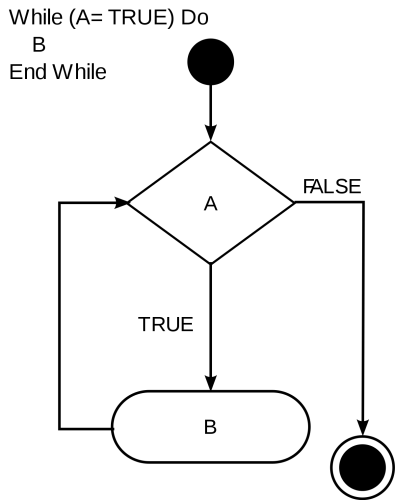
\includegraphics{figs/session_2/while-loop.png}
\caption{}
\end{figure}

    \begin{Verbatim}[commandchars=\\\{\}]
{\color{incolor}In [{\color{incolor}30}]:} \PY{n}{count} \PY{o}{=} \PY{l+m+mi}{0}
         \PY{k}{while} \PY{n}{count} \PY{o}{\PYZlt{}} \PY{l+m+mi}{5}\PY{p}{:}
             \PY{k}{print}\PY{p}{(}\PY{n}{count}\PY{p}{)}
             \PY{n}{count} \PY{o}{+}\PY{o}{=} \PY{l+m+mi}{1}  \PY{c+c1}{\PYZsh{} This is the same as count = count + 1}
\end{Verbatim}


    \begin{Verbatim}[commandchars=\\\{\}]
0
1
2
3
4

    \end{Verbatim}

    \begin{Verbatim}[commandchars=\\\{\}]
{\color{incolor}In [{\color{incolor} }]:} \PY{n}{input\PYZus{}text} \PY{o}{=} \PY{l+s+s2}{\PYZdq{}}\PY{l+s+s2}{run}\PY{l+s+s2}{\PYZdq{}}
        \PY{k}{while} \PY{n}{input\PYZus{}text} \PY{o}{!=} \PY{l+s+s2}{\PYZdq{}}\PY{l+s+s2}{exit}\PY{l+s+s2}{\PYZdq{}}\PY{p}{:}
            \PY{n}{input\PYZus{}text} \PY{o}{=} \PY{n+nb}{raw\PYZus{}input}\PY{p}{(}\PY{l+s+s2}{\PYZdq{}}\PY{l+s+s2}{Please type }\PY{l+s+s2}{\PYZsq{}}\PY{l+s+s2}{exit}\PY{l+s+s2}{\PYZsq{}}\PY{l+s+s2}{ to quit this program: }\PY{l+s+s2}{\PYZdq{}}\PY{p}{)}
        \PY{k}{print} \PY{l+s+s2}{\PYZdq{}}\PY{l+s+s2}{Quit !!!}\PY{l+s+s2}{\PYZdq{}}
\end{Verbatim}


    \subsection{"break" and "continue"
statements}\label{break-and-continue-statements}

\textbf{break} is used to \textbf{exit} a for loop or a while loop,
whereas \textbf{continue} is used to skip the current block, and return
to the "for" or "while" statement. A few examples:

    \begin{Verbatim}[commandchars=\\\{\}]
{\color{incolor}In [{\color{incolor}32}]:} \PY{n}{count} \PY{o}{=} \PY{l+m+mi}{0}
         \PY{k}{while} \PY{n+nb+bp}{True}\PY{p}{:}
             \PY{k}{print}\PY{p}{(}\PY{n}{count}\PY{p}{)}
             \PY{n}{count} \PY{o}{+}\PY{o}{=} \PY{l+m+mi}{1}
             \PY{k}{if} \PY{n}{count} \PY{o}{\PYZgt{}}\PY{o}{=} \PY{l+m+mi}{5}\PY{p}{:}
                 \PY{k}{break}
\end{Verbatim}


    \begin{Verbatim}[commandchars=\\\{\}]
0
1
2
3
4

    \end{Verbatim}

    \begin{Verbatim}[commandchars=\\\{\}]
{\color{incolor}In [{\color{incolor}33}]:} \PY{k}{for} \PY{n}{x} \PY{o+ow}{in} \PY{n+nb}{range}\PY{p}{(}\PY{l+m+mi}{10}\PY{p}{)}\PY{p}{:}
             \PY{c+c1}{\PYZsh{} Check if x is even}
             \PY{k}{if} \PY{n}{x} \PY{o}{\PYZpc{}} \PY{l+m+mi}{2} \PY{o}{==} \PY{l+m+mi}{0}\PY{p}{:}
                 \PY{k}{continue}
             \PY{k}{print}\PY{p}{(}\PY{n}{x}\PY{p}{)}
\end{Verbatim}


    \begin{Verbatim}[commandchars=\\\{\}]
1
3
5
7
9

    \end{Verbatim}

    \subsection{"Infinite loops" and break}\label{infinite-loops-and-break}

Sometimes you don't know it's time to end a loop until you get half way
through the body. In that case you can write an infinite loop on purpose
and then use the break statement to jump out of the loop.

    \subsection{Exercise}\label{exercise}

Ex1. Loop through and print out all even numbers from the numbers list
in the same order they are received. Don't print any numbers that come
after 237 in the sequence.

Hint: Using \texttt{loop}, \texttt{continue} and \texttt{break}

\begin{Shaded}
\begin{Highlighting}[]

\NormalTok{numbers }\OperatorTok{=}\NormalTok{ [}
    \DecValTok{951}\NormalTok{, }\DecValTok{402}\NormalTok{, }\DecValTok{984}\NormalTok{, }\DecValTok{651}\NormalTok{, }\DecValTok{360}\NormalTok{, }\DecValTok{69}\NormalTok{, }\DecValTok{408}\NormalTok{, }\DecValTok{319}\NormalTok{, }\DecValTok{601}\NormalTok{, }\DecValTok{485}\NormalTok{, }\DecValTok{980}\NormalTok{, }\DecValTok{507}\NormalTok{, }\DecValTok{725}\NormalTok{, }\DecValTok{547}\NormalTok{, }\DecValTok{544}\NormalTok{,}
    \DecValTok{615}\NormalTok{, }\DecValTok{83}\NormalTok{, }\DecValTok{165}\NormalTok{, }\DecValTok{141}\NormalTok{, }\DecValTok{501}\NormalTok{, }\DecValTok{263}\NormalTok{, }\DecValTok{617}\NormalTok{, }\DecValTok{865}\NormalTok{, }\DecValTok{575}\NormalTok{, }\DecValTok{219}\NormalTok{, }\DecValTok{390}\NormalTok{, }\DecValTok{984}\NormalTok{, }\DecValTok{592}\NormalTok{, }\DecValTok{236}\NormalTok{, }\DecValTok{105}\NormalTok{, }\DecValTok{942}\NormalTok{, }\DecValTok{941}\NormalTok{,}
    \DecValTok{386}\NormalTok{, }\DecValTok{462}\NormalTok{, }\DecValTok{47}\NormalTok{, }\DecValTok{418}\NormalTok{, }\DecValTok{907}\NormalTok{, }\DecValTok{344}\NormalTok{, }\DecValTok{236}\NormalTok{, }\DecValTok{375}\NormalTok{, }\DecValTok{823}\NormalTok{, }\DecValTok{566}\NormalTok{, }\DecValTok{597}\NormalTok{, }\DecValTok{978}\NormalTok{, }\DecValTok{328}\NormalTok{, }\DecValTok{615}\NormalTok{, }\DecValTok{953}\NormalTok{, }\DecValTok{345}\NormalTok{,}
    \DecValTok{399}\NormalTok{, }\DecValTok{162}\NormalTok{, }\DecValTok{758}\NormalTok{, }\DecValTok{219}\NormalTok{, }\DecValTok{918}\NormalTok{, }\DecValTok{237}\NormalTok{, }\DecValTok{412}\NormalTok{, }\DecValTok{566}\NormalTok{, }\DecValTok{826}\NormalTok{, }\DecValTok{248}\NormalTok{, }\DecValTok{866}\NormalTok{, }\DecValTok{950}\NormalTok{, }\DecValTok{626}\NormalTok{, }\DecValTok{949}\NormalTok{, }\DecValTok{687}\NormalTok{, }\DecValTok{217}\NormalTok{,}
    \DecValTok{815}\NormalTok{, }\DecValTok{67}\NormalTok{, }\DecValTok{104}\NormalTok{, }\DecValTok{58}\NormalTok{, }\DecValTok{512}\NormalTok{, }\DecValTok{24}\NormalTok{, }\DecValTok{892}\NormalTok{, }\DecValTok{894}\NormalTok{, }\DecValTok{767}\NormalTok{, }\DecValTok{553}\NormalTok{, }\DecValTok{81}\NormalTok{, }\DecValTok{379}\NormalTok{, }\DecValTok{843}\NormalTok{, }\DecValTok{831}\NormalTok{, }\DecValTok{445}\NormalTok{, }\DecValTok{742}\NormalTok{, }\DecValTok{717}\NormalTok{,}
    \DecValTok{958}\NormalTok{, }\DecValTok{609}\NormalTok{, }\DecValTok{842}\NormalTok{, }\DecValTok{451}\NormalTok{, }\DecValTok{688}\NormalTok{, }\DecValTok{753}\NormalTok{, }\DecValTok{854}\NormalTok{, }\DecValTok{685}\NormalTok{, }\DecValTok{93}\NormalTok{, }\DecValTok{857}\NormalTok{, }\DecValTok{440}\NormalTok{, }\DecValTok{380}\NormalTok{, }\DecValTok{126}\NormalTok{, }\DecValTok{721}\NormalTok{, }\DecValTok{328}\NormalTok{, }\DecValTok{753}\NormalTok{, }\DecValTok{470}\NormalTok{,}
    \DecValTok{743}\NormalTok{, }\DecValTok{527}
\NormalTok{]}

\CommentTok{# your code goes here}
\end{Highlighting}
\end{Shaded}

    \begin{Verbatim}[commandchars=\\\{\}]
{\color{incolor}In [{\color{incolor}10}]:} \PY{c+c1}{\PYZsh{} Solution}
         \PY{n}{numbers} \PY{o}{=} \PY{p}{[}
             \PY{l+m+mi}{951}\PY{p}{,} \PY{l+m+mi}{402}\PY{p}{,} \PY{l+m+mi}{984}\PY{p}{,} \PY{l+m+mi}{651}\PY{p}{,} \PY{l+m+mi}{360}\PY{p}{,} \PY{l+m+mi}{69}\PY{p}{,} \PY{l+m+mi}{408}\PY{p}{,} \PY{l+m+mi}{319}\PY{p}{,} \PY{l+m+mi}{601}\PY{p}{,} \PY{l+m+mi}{485}\PY{p}{,} \PY{l+m+mi}{980}\PY{p}{,} \PY{l+m+mi}{507}\PY{p}{,} \PY{l+m+mi}{725}\PY{p}{,} \PY{l+m+mi}{547}\PY{p}{,} \PY{l+m+mi}{544}\PY{p}{,}
             \PY{l+m+mi}{615}\PY{p}{,} \PY{l+m+mi}{83}\PY{p}{,} \PY{l+m+mi}{165}\PY{p}{,} \PY{l+m+mi}{141}\PY{p}{,} \PY{l+m+mi}{501}\PY{p}{,} \PY{l+m+mi}{263}\PY{p}{,} \PY{l+m+mi}{617}\PY{p}{,} \PY{l+m+mi}{865}\PY{p}{,} \PY{l+m+mi}{575}\PY{p}{,} \PY{l+m+mi}{219}\PY{p}{,} \PY{l+m+mi}{390}\PY{p}{,} \PY{l+m+mi}{984}\PY{p}{,} \PY{l+m+mi}{592}\PY{p}{,} \PY{l+m+mi}{236}\PY{p}{,} \PY{l+m+mi}{105}\PY{p}{,} \PY{l+m+mi}{942}\PY{p}{,} \PY{l+m+mi}{941}\PY{p}{,}
             \PY{l+m+mi}{386}\PY{p}{,} \PY{l+m+mi}{462}\PY{p}{,} \PY{l+m+mi}{47}\PY{p}{,} \PY{l+m+mi}{418}\PY{p}{,} \PY{l+m+mi}{907}\PY{p}{,} \PY{l+m+mi}{344}\PY{p}{,} \PY{l+m+mi}{236}\PY{p}{,} \PY{l+m+mi}{375}\PY{p}{,} \PY{l+m+mi}{823}\PY{p}{,} \PY{l+m+mi}{566}\PY{p}{,} \PY{l+m+mi}{597}\PY{p}{,} \PY{l+m+mi}{978}\PY{p}{,} \PY{l+m+mi}{328}\PY{p}{,} \PY{l+m+mi}{615}\PY{p}{,} \PY{l+m+mi}{953}\PY{p}{,} \PY{l+m+mi}{345}\PY{p}{,}
             \PY{l+m+mi}{399}\PY{p}{,} \PY{l+m+mi}{162}\PY{p}{,} \PY{l+m+mi}{758}\PY{p}{,} \PY{l+m+mi}{219}\PY{p}{,} \PY{l+m+mi}{918}\PY{p}{,} \PY{l+m+mi}{237}\PY{p}{,} \PY{l+m+mi}{412}\PY{p}{,} \PY{l+m+mi}{566}\PY{p}{,} \PY{l+m+mi}{826}\PY{p}{,} \PY{l+m+mi}{248}\PY{p}{,} \PY{l+m+mi}{866}\PY{p}{,} \PY{l+m+mi}{950}\PY{p}{,} \PY{l+m+mi}{626}\PY{p}{,} \PY{l+m+mi}{949}\PY{p}{,} \PY{l+m+mi}{687}\PY{p}{,} \PY{l+m+mi}{217}\PY{p}{,}
             \PY{l+m+mi}{815}\PY{p}{,} \PY{l+m+mi}{67}\PY{p}{,} \PY{l+m+mi}{104}\PY{p}{,} \PY{l+m+mi}{58}\PY{p}{,} \PY{l+m+mi}{512}\PY{p}{,} \PY{l+m+mi}{24}\PY{p}{,} \PY{l+m+mi}{892}\PY{p}{,} \PY{l+m+mi}{894}\PY{p}{,} \PY{l+m+mi}{767}\PY{p}{,} \PY{l+m+mi}{553}\PY{p}{,} \PY{l+m+mi}{81}\PY{p}{,} \PY{l+m+mi}{379}\PY{p}{,} \PY{l+m+mi}{843}\PY{p}{,} \PY{l+m+mi}{831}\PY{p}{,} \PY{l+m+mi}{445}\PY{p}{,} \PY{l+m+mi}{742}\PY{p}{,} \PY{l+m+mi}{717}\PY{p}{,}
             \PY{l+m+mi}{958}\PY{p}{,} \PY{l+m+mi}{609}\PY{p}{,} \PY{l+m+mi}{842}\PY{p}{,} \PY{l+m+mi}{451}\PY{p}{,} \PY{l+m+mi}{688}\PY{p}{,} \PY{l+m+mi}{753}\PY{p}{,} \PY{l+m+mi}{854}\PY{p}{,} \PY{l+m+mi}{685}\PY{p}{,} \PY{l+m+mi}{93}\PY{p}{,} \PY{l+m+mi}{857}\PY{p}{,} \PY{l+m+mi}{440}\PY{p}{,} \PY{l+m+mi}{380}\PY{p}{,} \PY{l+m+mi}{126}\PY{p}{,} \PY{l+m+mi}{721}\PY{p}{,} \PY{l+m+mi}{328}\PY{p}{,} \PY{l+m+mi}{753}\PY{p}{,} \PY{l+m+mi}{470}\PY{p}{,}
             \PY{l+m+mi}{743}\PY{p}{,} \PY{l+m+mi}{527}
         \PY{p}{]}
         
         \PY{k}{for} \PY{n}{n} \PY{o+ow}{in} \PY{n}{numbers}\PY{p}{:}
             \PY{k}{if} \PY{n}{n} \PY{o}{==} \PY{l+m+mi}{237}\PY{p}{:}
                 \PY{k}{break}
             \PY{k}{if} \PY{n}{n} \PY{o}{\PYZpc{}} \PY{l+m+mi}{2} \PY{o}{==} \PY{l+m+mi}{0}\PY{p}{:}
                 \PY{k}{continue}
             \PY{k}{print} \PY{n}{n}\PY{p}{,} 
\end{Verbatim}


    \begin{Verbatim}[commandchars=\\\{\}]
951 651 69 319 601 485 507 725 547 615 83 165 141 501 263 617 865 575 219 105 941 47 907 375 823 597 615 953 345 399 219

    \end{Verbatim}

    Ex2. \textbf{Faces on Money}

It is common for images of a country's previous leaders, or other
individuals of historical significance, to appear on its money. The
individuals that appear on banknotes in the United States are listed in
the table bellow.

\begin{longtable}[]{@{}ll@{}}
\toprule
Individual & Amount\tabularnewline
\midrule
\endhead
George Washington & \$1\tabularnewline
Thomas Jefferson & \$2\tabularnewline
Abraham Lincoln & \$5\tabularnewline
Alexander Hamilton & \$10\tabularnewline
Andrew Jackson & \$20\tabularnewline
Ulysses S. Grant & \$50\tabularnewline
Benjamin Frankli & \$100\tabularnewline
\bottomrule
\end{longtable}

Write a program that begins by reading the denomination of a banknote
from the user. Then your program should display the name of the
individual that appears on the banknote of the entered amount. An
appropriate error message should be displayed if no such note exists.

    \begin{Verbatim}[commandchars=\\\{\}]
{\color{incolor}In [{\color{incolor}1}]:} \PY{c+c1}{\PYZsh{} Solution}
        \PY{n}{banknotes} \PY{o}{=} \PY{p}{\PYZob{}}
            \PY{l+m+mi}{1}\PY{p}{:} \PY{l+s+s1}{\PYZsq{}}\PY{l+s+s1}{George Washington}\PY{l+s+s1}{\PYZsq{}}\PY{p}{,}
            \PY{l+m+mi}{2}\PY{p}{:} \PY{l+s+s1}{\PYZsq{}}\PY{l+s+s1}{Thomas Jefferson}\PY{l+s+s1}{\PYZsq{}}\PY{p}{,}
            \PY{l+m+mi}{5}\PY{p}{:} \PY{l+s+s1}{\PYZsq{}}\PY{l+s+s1}{Abraham Lincoln}\PY{l+s+s1}{\PYZsq{}}\PY{p}{,}
            \PY{l+m+mi}{10}\PY{p}{:} \PY{l+s+s1}{\PYZsq{}}\PY{l+s+s1}{Alexander Hamilton}\PY{l+s+s1}{\PYZsq{}}\PY{p}{,}
            \PY{l+m+mi}{20}\PY{p}{:} \PY{l+s+s1}{\PYZsq{}}\PY{l+s+s1}{Andrew Jackson}\PY{l+s+s1}{\PYZsq{}}\PY{p}{,}
            \PY{l+m+mi}{50}\PY{p}{:} \PY{l+s+s1}{\PYZsq{}}\PY{l+s+s1}{Ulysses S. Grant}\PY{l+s+s1}{\PYZsq{}}\PY{p}{,}
            \PY{l+m+mi}{100}\PY{p}{:} \PY{l+s+s1}{\PYZsq{}}\PY{l+s+s1}{Benjamin Frankli}\PY{l+s+s1}{\PYZsq{}}
        \PY{p}{\PYZcb{}}
        
        \PY{c+c1}{\PYZsh{} reading the denomination of a banknote}
        \PY{n}{amount} \PY{o}{=} \PY{n+nb}{int}\PY{p}{(}\PY{n+nb}{input}\PY{p}{(}\PY{l+s+s2}{\PYZdq{}}\PY{l+s+s2}{Please enter amount: }\PY{l+s+s2}{\PYZdq{}}\PY{p}{)}\PY{p}{)}
        
        \PY{k}{while} \PY{n}{amount} \PY{o}{\PYZgt{}} \PY{l+m+mi}{0}\PY{p}{:}
            \PY{k}{if} \PY{n}{amount} \PY{o}{/} \PY{l+m+mi}{100} \PY{o}{\PYZgt{}} \PY{l+m+mi}{0}\PY{p}{:}
                \PY{k}{print} \PY{p}{(}\PY{n}{amount} \PY{o}{/} \PY{l+m+mi}{100}\PY{p}{)}\PY{p}{,} \PY{l+s+s1}{\PYZsq{}}\PY{l+s+s1}{ x }\PY{l+s+s1}{\PYZsq{}}\PY{p}{,} \PY{n}{banknotes}\PY{p}{[}\PY{l+m+mi}{100}\PY{p}{]}\PY{p}{,} \PY{l+s+s1}{\PYZsq{}}\PY{l+s+s1}{(\PYZdl{}100)}\PY{l+s+s1}{\PYZsq{}}
                \PY{n}{amount} \PY{o}{=} \PY{n}{amount} \PY{o}{\PYZpc{}} \PY{l+m+mi}{100}
            \PY{k}{if} \PY{n}{amount} \PY{o}{/} \PY{l+m+mi}{50} \PY{o}{\PYZgt{}} \PY{l+m+mi}{0}\PY{p}{:}
                \PY{k}{print} \PY{p}{(}\PY{n}{amount} \PY{o}{/} \PY{l+m+mi}{50}\PY{p}{)}\PY{p}{,} \PY{l+s+s1}{\PYZsq{}}\PY{l+s+s1}{ x }\PY{l+s+s1}{\PYZsq{}}\PY{p}{,} \PY{n}{banknotes}\PY{p}{[}\PY{l+m+mi}{50}\PY{p}{]}\PY{p}{,} \PY{l+s+s1}{\PYZsq{}}\PY{l+s+s1}{(\PYZdl{}50)}\PY{l+s+s1}{\PYZsq{}}
                \PY{n}{amount} \PY{o}{=} \PY{n}{amount} \PY{o}{\PYZpc{}} \PY{l+m+mi}{50}   
            \PY{k}{if} \PY{n}{amount} \PY{o}{/} \PY{l+m+mi}{20} \PY{o}{\PYZgt{}} \PY{l+m+mi}{0}\PY{p}{:}
                \PY{k}{print} \PY{p}{(}\PY{n}{amount} \PY{o}{/} \PY{l+m+mi}{20}\PY{p}{)}\PY{p}{,} \PY{l+s+s1}{\PYZsq{}}\PY{l+s+s1}{ x }\PY{l+s+s1}{\PYZsq{}}\PY{p}{,} \PY{n}{banknotes}\PY{p}{[}\PY{l+m+mi}{20}\PY{p}{]}\PY{p}{,} \PY{l+s+s1}{\PYZsq{}}\PY{l+s+s1}{(\PYZdl{}20)}\PY{l+s+s1}{\PYZsq{}}
                \PY{n}{amount} \PY{o}{=} \PY{n}{amount} \PY{o}{\PYZpc{}} \PY{l+m+mi}{20}
            \PY{k}{if} \PY{n}{amount} \PY{o}{/} \PY{l+m+mi}{10} \PY{o}{\PYZgt{}} \PY{l+m+mi}{0}\PY{p}{:}
                \PY{k}{print} \PY{p}{(}\PY{n}{amount} \PY{o}{/} \PY{l+m+mi}{10}\PY{p}{)}\PY{p}{,} \PY{l+s+s1}{\PYZsq{}}\PY{l+s+s1}{ x }\PY{l+s+s1}{\PYZsq{}}\PY{p}{,} \PY{n}{banknotes}\PY{p}{[}\PY{l+m+mi}{10}\PY{p}{]}\PY{p}{,} \PY{l+s+s1}{\PYZsq{}}\PY{l+s+s1}{(\PYZdl{}10)}\PY{l+s+s1}{\PYZsq{}}
                \PY{n}{amount} \PY{o}{=} \PY{n}{amount} \PY{o}{\PYZpc{}} \PY{l+m+mi}{10}
            \PY{k}{if} \PY{n}{amount} \PY{o}{/} \PY{l+m+mi}{5} \PY{o}{\PYZgt{}} \PY{l+m+mi}{0}\PY{p}{:}
                \PY{k}{print} \PY{p}{(}\PY{n}{amount} \PY{o}{/} \PY{l+m+mi}{5}\PY{p}{)}\PY{p}{,} \PY{l+s+s1}{\PYZsq{}}\PY{l+s+s1}{ x }\PY{l+s+s1}{\PYZsq{}}\PY{p}{,} \PY{n}{banknotes}\PY{p}{[}\PY{l+m+mi}{5}\PY{p}{]}\PY{p}{,} \PY{l+s+s1}{\PYZsq{}}\PY{l+s+s1}{(\PYZdl{}5)}\PY{l+s+s1}{\PYZsq{}}
                \PY{n}{amount} \PY{o}{=} \PY{n}{amount} \PY{o}{\PYZpc{}} \PY{l+m+mi}{5}
            \PY{k}{if} \PY{n}{amount} \PY{o}{/} \PY{l+m+mi}{2} \PY{o}{\PYZgt{}} \PY{l+m+mi}{0}\PY{p}{:}
                \PY{k}{print} \PY{p}{(}\PY{n}{amount} \PY{o}{/} \PY{l+m+mi}{2}\PY{p}{)}\PY{p}{,} \PY{l+s+s1}{\PYZsq{}}\PY{l+s+s1}{ x }\PY{l+s+s1}{\PYZsq{}}\PY{p}{,} \PY{n}{banknotes}\PY{p}{[}\PY{l+m+mi}{2}\PY{p}{]}\PY{p}{,} \PY{l+s+s1}{\PYZsq{}}\PY{l+s+s1}{(\PYZdl{}2)}\PY{l+s+s1}{\PYZsq{}}
                \PY{n}{amount} \PY{o}{=} \PY{n}{amount} \PY{o}{\PYZpc{}} \PY{l+m+mi}{2}
            \PY{k}{if} \PY{n}{amount} \PY{o}{/} \PY{l+m+mi}{1} \PY{o}{\PYZgt{}} \PY{l+m+mi}{0}\PY{p}{:}
                \PY{k}{print} \PY{p}{(}\PY{n}{amount} \PY{o}{/} \PY{l+m+mi}{1}\PY{p}{)}\PY{p}{,} \PY{l+s+s1}{\PYZsq{}}\PY{l+s+s1}{ x }\PY{l+s+s1}{\PYZsq{}}\PY{p}{,} \PY{n}{banknotes}\PY{p}{[}\PY{l+m+mi}{1}\PY{p}{]}\PY{p}{,} \PY{l+s+s1}{\PYZsq{}}\PY{l+s+s1}{(\PYZdl{}1)}\PY{l+s+s1}{\PYZsq{}}
                \PY{n}{amount} \PY{o}{=} \PY{n}{amount} \PY{o}{\PYZpc{}} \PY{l+m+mi}{1}
\end{Verbatim}


    \begin{Verbatim}[commandchars=\\\{\}]
Please enter amount: 345
3  x  Benjamin Frankli (\$100)
2  x  Andrew Jackson (\$20)
1  x  Abraham Lincoln (\$5)

    \end{Verbatim}

    \begin{Verbatim}[commandchars=\\\{\}]
{\color{incolor}In [{\color{incolor}16}]:} \PY{c+c1}{\PYZsh{} Solution for shorter}
         
         \PY{n}{banknotes} \PY{o}{=} \PY{p}{\PYZob{}}
             \PY{l+m+mi}{1}\PY{p}{:} \PY{l+s+s1}{\PYZsq{}}\PY{l+s+s1}{George Washington}\PY{l+s+s1}{\PYZsq{}}\PY{p}{,}
             \PY{l+m+mi}{2}\PY{p}{:} \PY{l+s+s1}{\PYZsq{}}\PY{l+s+s1}{Thomas Jefferson}\PY{l+s+s1}{\PYZsq{}}\PY{p}{,}
             \PY{l+m+mi}{5}\PY{p}{:} \PY{l+s+s1}{\PYZsq{}}\PY{l+s+s1}{Abraham Lincoln}\PY{l+s+s1}{\PYZsq{}}\PY{p}{,}
             \PY{l+m+mi}{10}\PY{p}{:} \PY{l+s+s1}{\PYZsq{}}\PY{l+s+s1}{Alexander Hamilton}\PY{l+s+s1}{\PYZsq{}}\PY{p}{,}
             \PY{l+m+mi}{20}\PY{p}{:} \PY{l+s+s1}{\PYZsq{}}\PY{l+s+s1}{Andrew Jackson}\PY{l+s+s1}{\PYZsq{}}\PY{p}{,}
             \PY{l+m+mi}{50}\PY{p}{:} \PY{l+s+s1}{\PYZsq{}}\PY{l+s+s1}{Ulysses S. Grant}\PY{l+s+s1}{\PYZsq{}}\PY{p}{,}
             \PY{l+m+mi}{100}\PY{p}{:} \PY{l+s+s1}{\PYZsq{}}\PY{l+s+s1}{Benjamin Frankli}\PY{l+s+s1}{\PYZsq{}}
         \PY{p}{\PYZcb{}}
         
         \PY{c+c1}{\PYZsh{} reading the denomination of a banknote}
         \PY{n}{amount} \PY{o}{=} \PY{n+nb}{int}\PY{p}{(}\PY{n+nb}{input}\PY{p}{(}\PY{l+s+s2}{\PYZdq{}}\PY{l+s+s2}{Please enter amount: }\PY{l+s+s2}{\PYZdq{}}\PY{p}{)}\PY{p}{)}
         
         \PY{k}{while} \PY{n}{amount} \PY{o}{\PYZgt{}} \PY{l+m+mi}{0}\PY{p}{:}
             \PY{k}{for} \PY{n}{i} \PY{o+ow}{in} \PY{n+nb}{sorted}\PY{p}{(}\PY{n}{banknotes}\PY{o}{.}\PY{n}{keys}\PY{p}{(}\PY{p}{)}\PY{p}{,} \PY{n}{reverse}\PY{o}{=}\PY{n+nb+bp}{True}\PY{p}{)}\PY{p}{:}
                 \PY{k}{if} \PY{n}{amount} \PY{o}{/} \PY{n}{i} \PY{o}{\PYZgt{}} \PY{l+m+mi}{0}\PY{p}{:}
                     \PY{k}{print} \PY{p}{(}\PY{n}{amount} \PY{o}{/} \PY{n}{i}\PY{p}{)}\PY{p}{,} \PY{l+s+s1}{\PYZsq{}}\PY{l+s+s1}{ x }\PY{l+s+s1}{\PYZsq{}}\PY{p}{,} \PY{n}{banknotes}\PY{p}{[}\PY{n}{i}\PY{p}{]}\PY{p}{,} \PY{l+s+s1}{\PYZsq{}}\PY{l+s+s1}{(\PYZdl{}}\PY{l+s+s1}{\PYZsq{}}\PY{o}{+}\PY{n+nb}{str}\PY{p}{(}\PY{n}{i}\PY{p}{)}\PY{o}{+}\PY{l+s+s1}{\PYZsq{}}\PY{l+s+s1}{)}\PY{l+s+s1}{\PYZsq{}}
                     \PY{n}{amount} \PY{o}{=} \PY{n}{amount} \PY{o}{\PYZpc{}} \PY{n}{i}
                     \PY{k}{break}
\end{Verbatim}


    \begin{Verbatim}[commandchars=\\\{\}]
Please enter amount: 456
4  x  Benjamin Frankli (\$100)
1  x  Ulysses S. Grant (\$50)
1  x  Abraham Lincoln (\$5)
1  x  George Washington (\$1)

    \end{Verbatim}

    Ex3. (Bonus) Implement insertion sort in Python.

\begin{Shaded}
\begin{Highlighting}[]
\NormalTok{insertion_sort([}\DecValTok{3}\NormalTok{,}\DecValTok{4}\NormalTok{,}\DecValTok{6}\NormalTok{,}\DecValTok{7}\NormalTok{,}\DecValTok{1}\NormalTok{])}
\end{Highlighting}
\end{Shaded}

    Ex4. (Bonus) Implement selection sort in Python.

\begin{Shaded}
\begin{Highlighting}[]
\NormalTok{selection_sort([}\DecValTok{3}\NormalTok{,}\DecValTok{4}\NormalTok{,}\DecValTok{6}\NormalTok{,}\DecValTok{7}\NormalTok{,}\DecValTok{1}\NormalTok{])}
\end{Highlighting}
\end{Shaded}

    \section{References}\label{references}

\begin{itemize}
\tightlist
\item
  Class and Object:
  \url{https://www.learnpython.org/en/Classes_and_Objects}
\item
  Learn Python - Loop: \url{https://www.learnpython.org/en/Loops}
\item
  http://www.afterhoursprogramming.com/tutorial/Python/If-Statement/
\item
  http://www.afterhoursprogramming.com/tutorial/Python/Classes/
\end{itemize}


    % Add a bibliography block to the postdoc
    
    
    
    \end{document}
